% =============================
% ภาคผนวก
% =============================
% หมายเหตุ: ก่อนเริ่มภาคผนวก ระบบจะสร้างหน้าคั่นให้อัตโนมัติ
% ใช้คำสั่ง \appendiceschapter{ชื่อภาคผนวก} สำหรับแต่ละภาคผนวก
% ระบบจะกำหนดตัวอักษร ก, ข, ค ... ให้โดยอัตโนมัติ
%
% *** ลบข้อความตัวอย่างด้านล่าง แล้วใส่ภาพ UI / Prototype ของตนเอง ***

% =============================
% ภาคผนวก ก
% =============================
\setcounter{chapter}{-1}
\appendiceschapter{ตัวอย่าง UI หรือ Prototype}

\section*{ผลการพัฒนาแอปพลิเคชัน}

ภาคผนวกนี้แสดงภาพหน้าจอของแอปพลิเคชันต้นแบบ Pacegasus ซึ่งพัฒนาขึ้นตามลำดับการใช้งานจริง ตั้งแต่การเข้าสู่ระบบ การกรอกข้อมูล การเลือกแผนการฝึก การวิ่ง และการรับรางวัล

\subsection*{การเข้าสู่ระบบและการสมัครสมาชิก}

หน้าจอเข้าสู่ระบบรองรับการกรอกอีเมลและการเข้าสู่ระบบด้วย Google ส่วนหน้าจอสมัครสมาชิกช่วยให้ผู้ใช้สร้างบัญชีใหม่ รวมถึงหน้าข้อกำหนดและการยินยอม และหน้าสำหรับยืนยันตัวตนด้วยรหัส OTP

\begin{figure}[H]\centering
\begin{subfigure}[t]{0.31\textwidth}\centering
\includegraphics[width=\textwidth]{images/pegasus-login.png}\caption{เข้าสู่ระบบ}\end{subfigure}\hfill
\begin{subfigure}[t]{0.31\textwidth}\centering
\includegraphics[width=\textwidth]{images/pegasus-sign-up.png}\caption{สมัครสมาชิก}\end{subfigure}\hfill
\begin{subfigure}[t]{0.31\textwidth}\centering
\includegraphics[width=\textwidth]{images/pegasus-otp-verification.png}\caption{ยืนยัน OTP}\end{subfigure}
\caption{หน้าจอการเข้าสู่ระบบและการสมัครสมาชิก}\label{fig:app-auth}
\end{figure}

\begin{figure}[H]\centering
\begin{subfigure}[t]{0.31\textwidth}\centering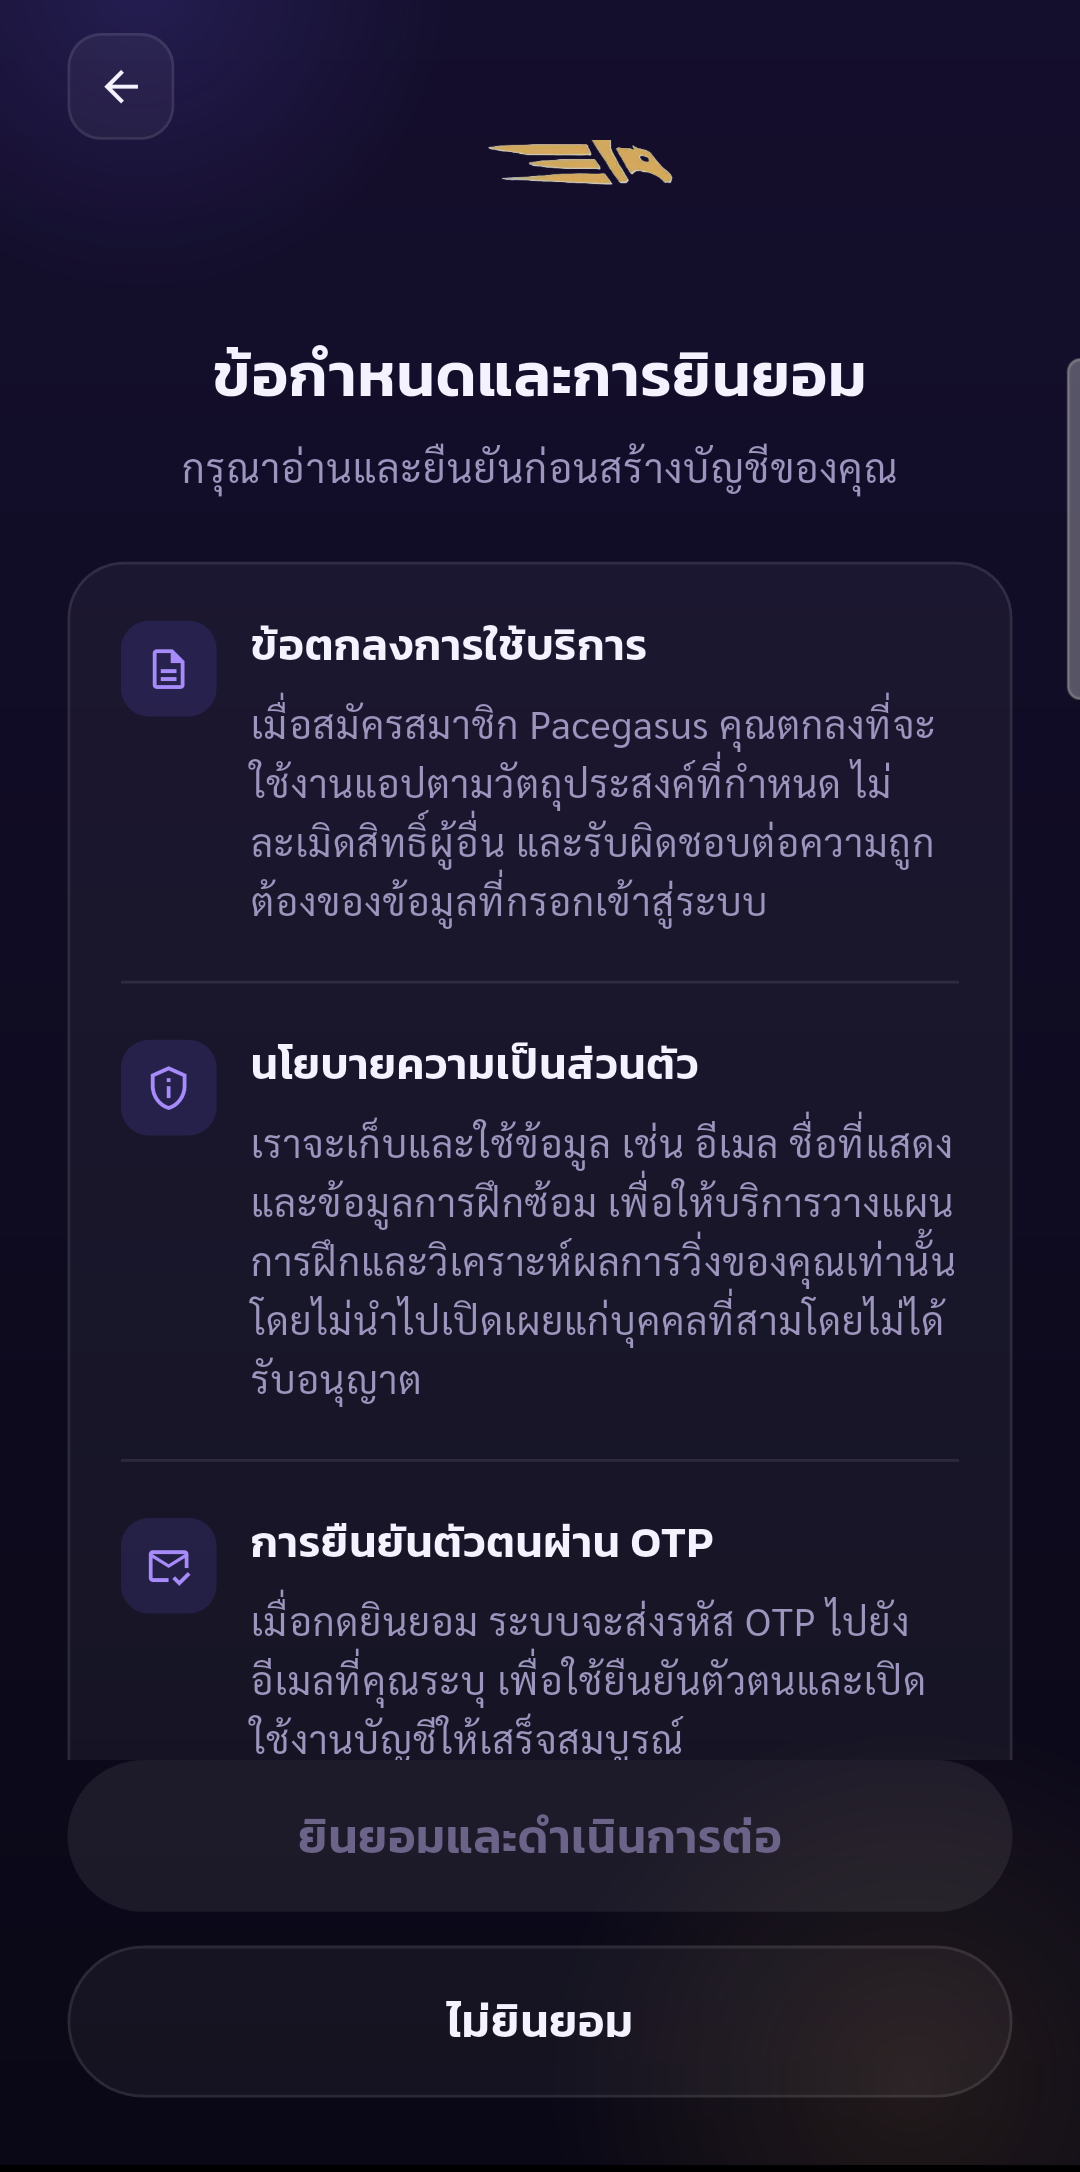
\includegraphics[width=\textwidth]{images/pegasus-terms-and-consent-unchecked.png}\caption{ยังไม่ยินยอม}\end{subfigure}\hfill
\begin{subfigure}[t]{0.31\textwidth}\centering
\includegraphics[width=\textwidth]{images/pegasus-terms-and-consent-checked.png}\caption{ยินยอมแล้ว}\end{subfigure}
\caption{หน้าข้อกำหนดและการยินยอม}\label{fig:app-consent}
\end{figure}

\subsection*{การเก็บข้อมูลพื้นฐานและข้อมูลสุขภาพ}

ขั้นตอน Onboarding ประกอบด้วยการกรอกข้อมูลพื้นฐาน ประวัติการวิ่ง และข้อมูลสุขภาพ เพื่อให้ระบบนำไปประกอบการวางแผนการฝึก

\begin{figure}[H]\centering
\begin{subfigure}[t]{0.31\textwidth}\centering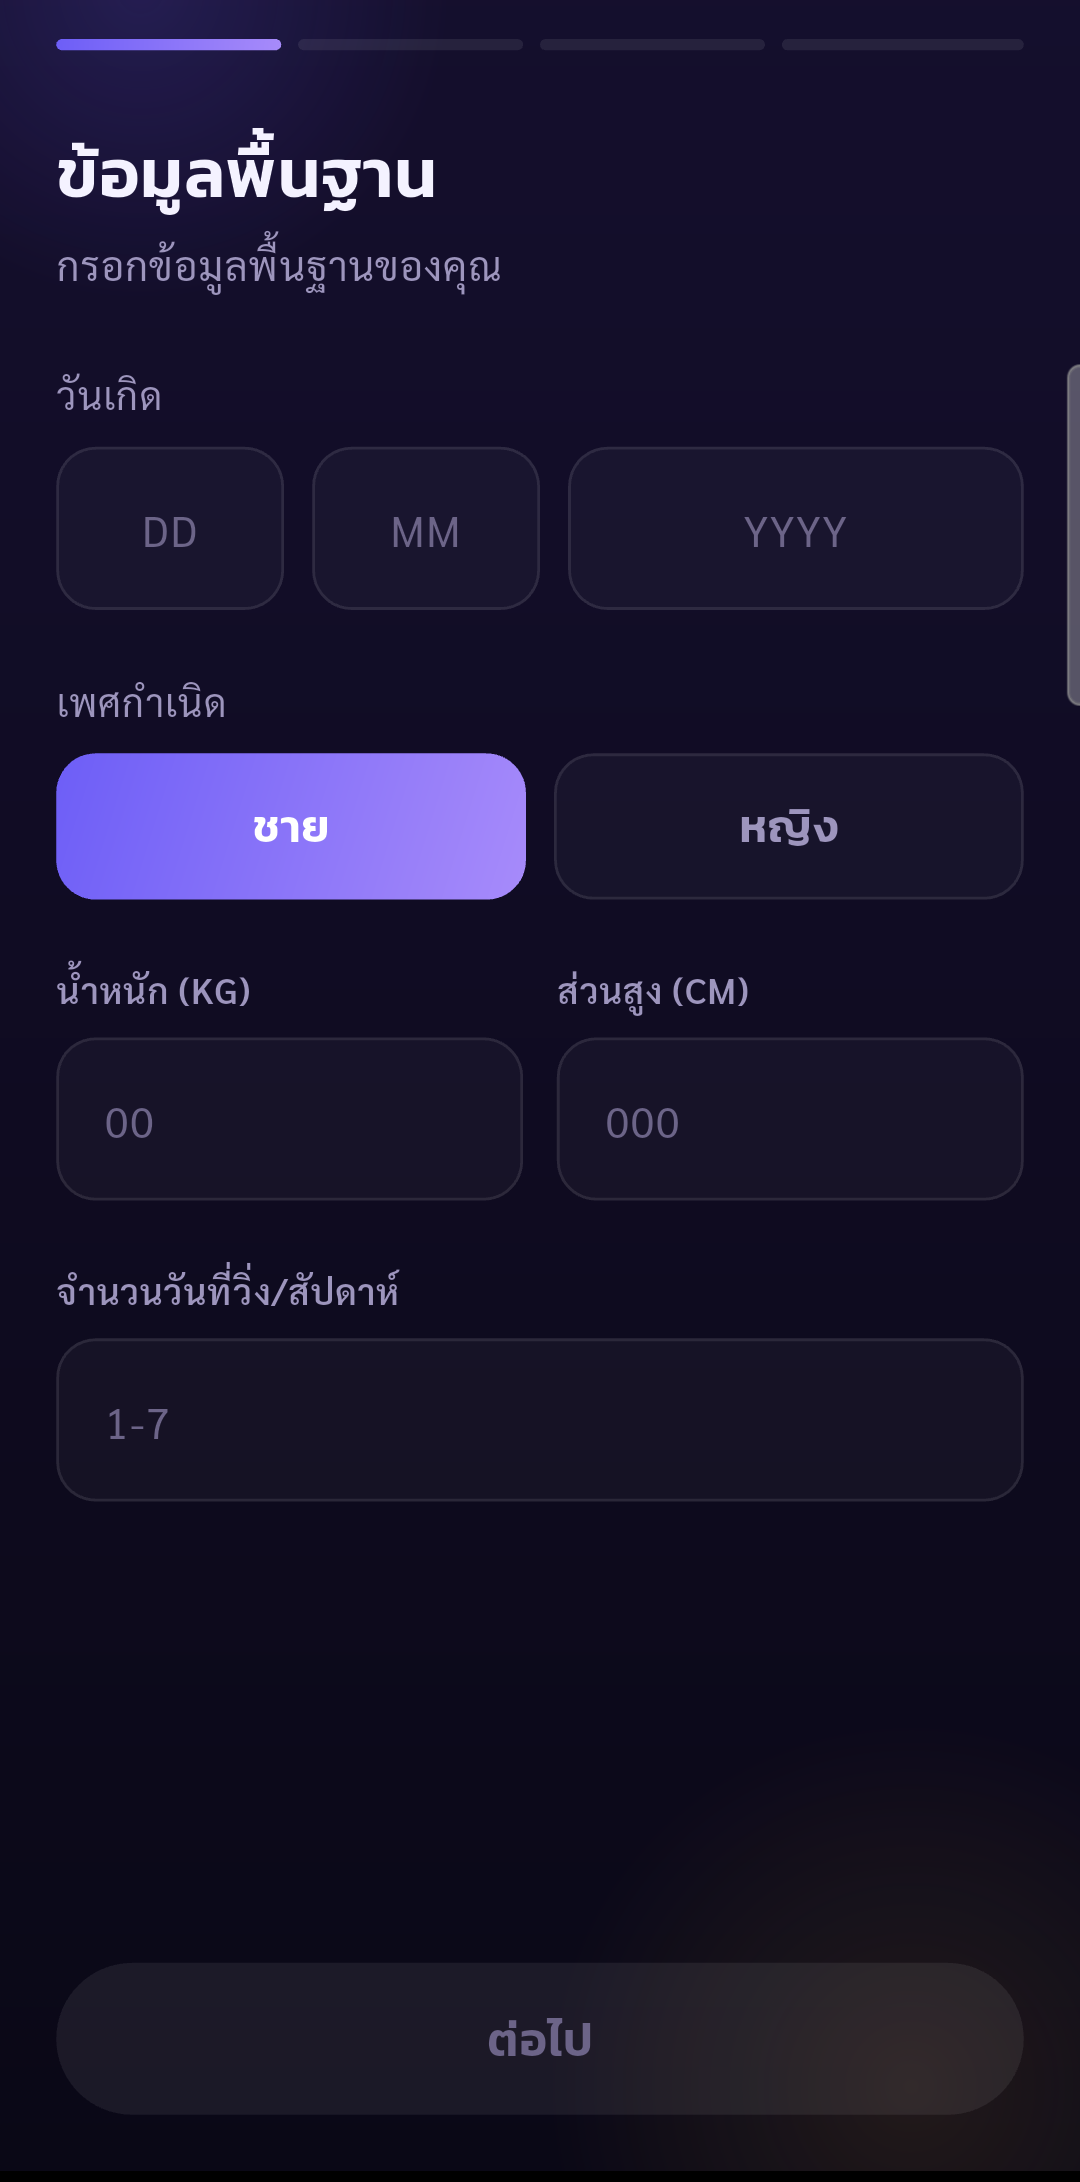
\includegraphics[width=\textwidth]{images/pegasus-onboarding-basic-information.png}\caption{ข้อมูลพื้นฐาน}\end{subfigure}\hfill
\begin{subfigure}[t]{0.31\textwidth}\centering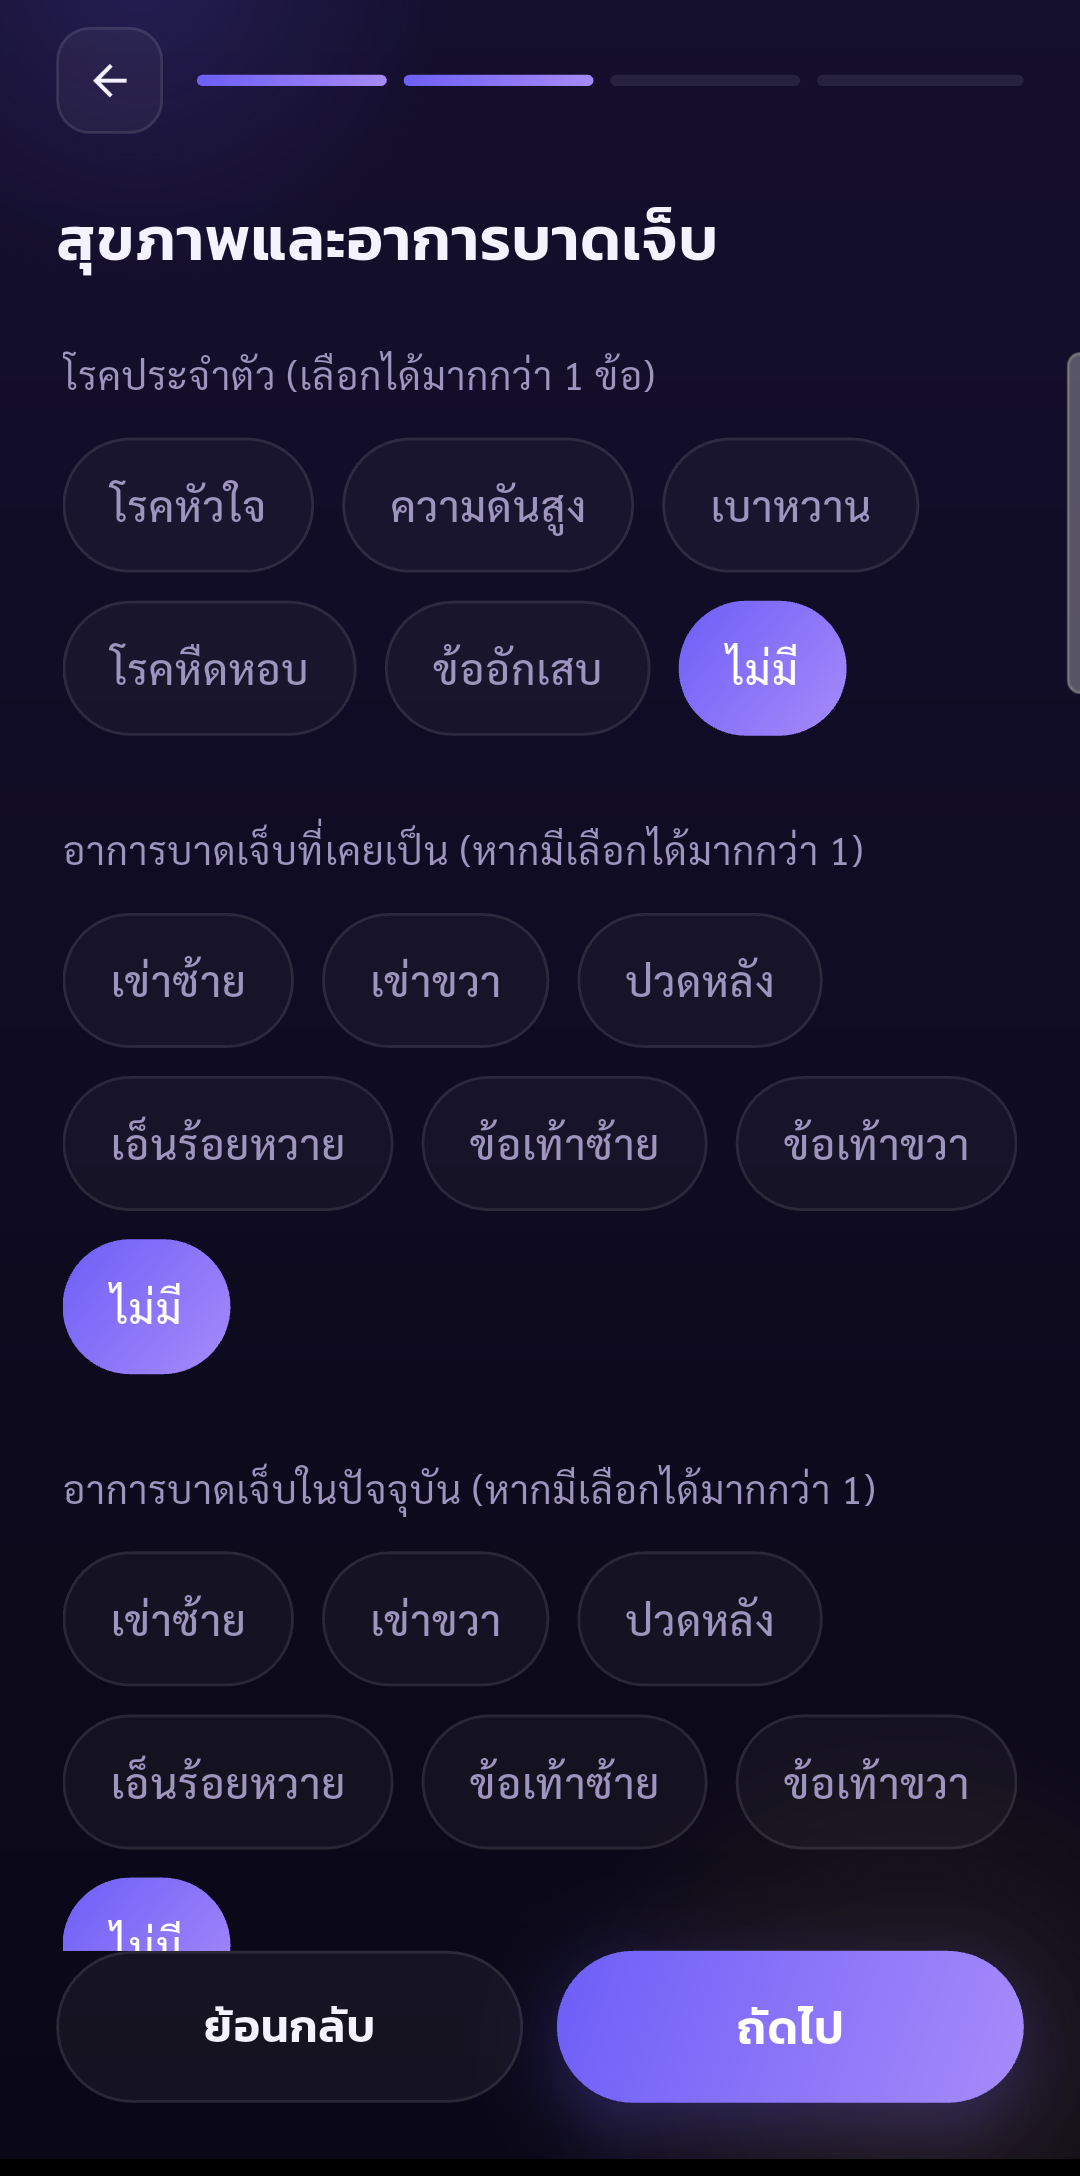
\includegraphics[width=\textwidth]{images/pegasus-onboarding-health-and-injuries.png}\caption{สุขภาพและอาการบาดเจ็บ}\end{subfigure}\hfill
\begin{subfigure}[t]{0.31\textwidth}\centering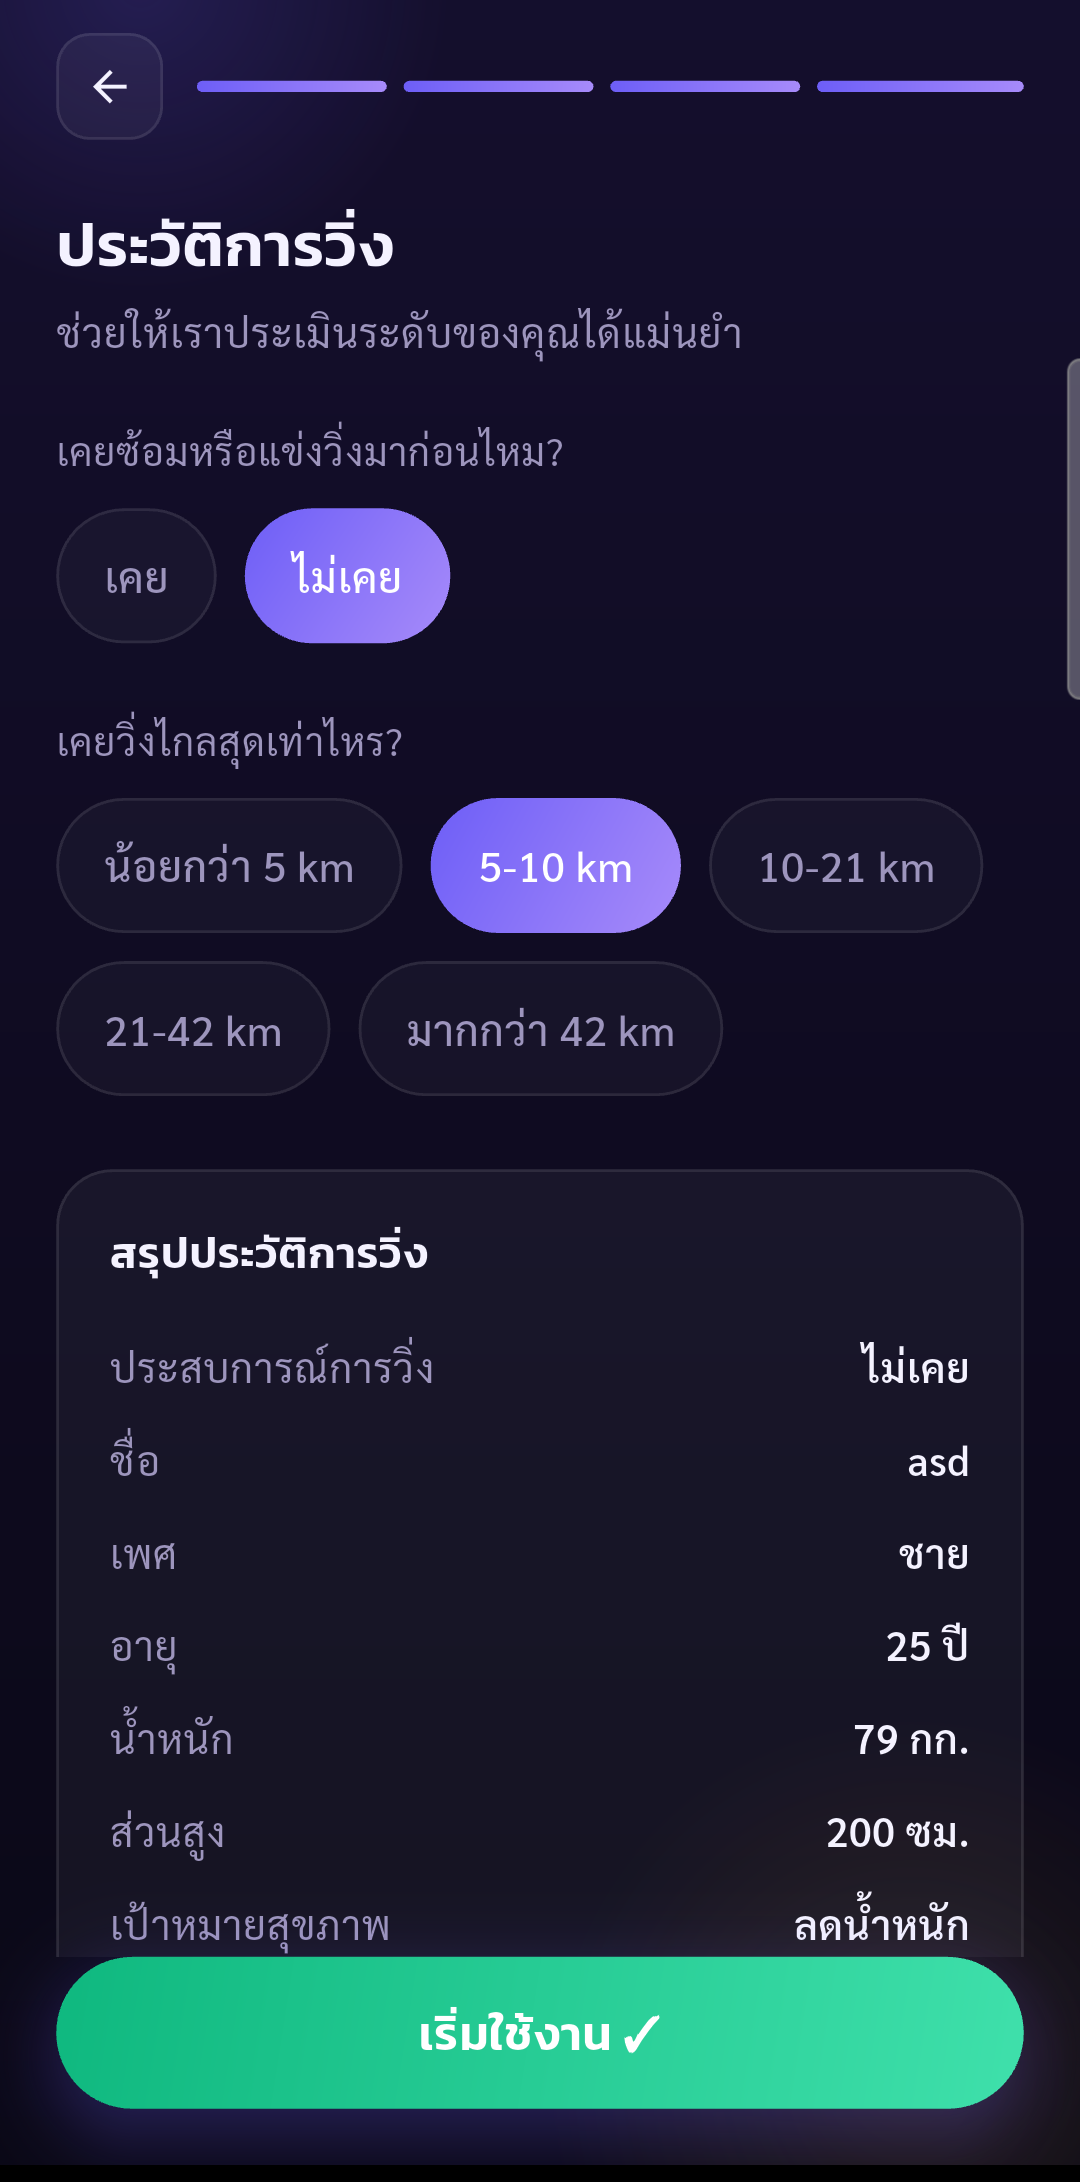
\includegraphics[width=\textwidth]{images/pegasus-onboarding-running-history-summary.png}\caption{ประวัติการวิ่ง}\end{subfigure}
\caption{หน้าจอการเก็บข้อมูลสำหรับสร้างโปรไฟล์ผู้ใช้}\label{fig:app-onboarding}
\end{figure}

\subsection*{การกำหนดเป้าหมายและการเลือกแผนการฝึก}

ผู้ใช้สามารถเลือกเป้าหมายด้านระยะทางและเป้าหมายด้านสุขภาพ ระบบจะใช้ข้อมูลดังกล่าวเป็นเงื่อนไขเริ่มต้นของ Adaptive Training Engine

\begin{figure}[H]\centering
\begin{subfigure}[t]{0.31\textwidth}\centering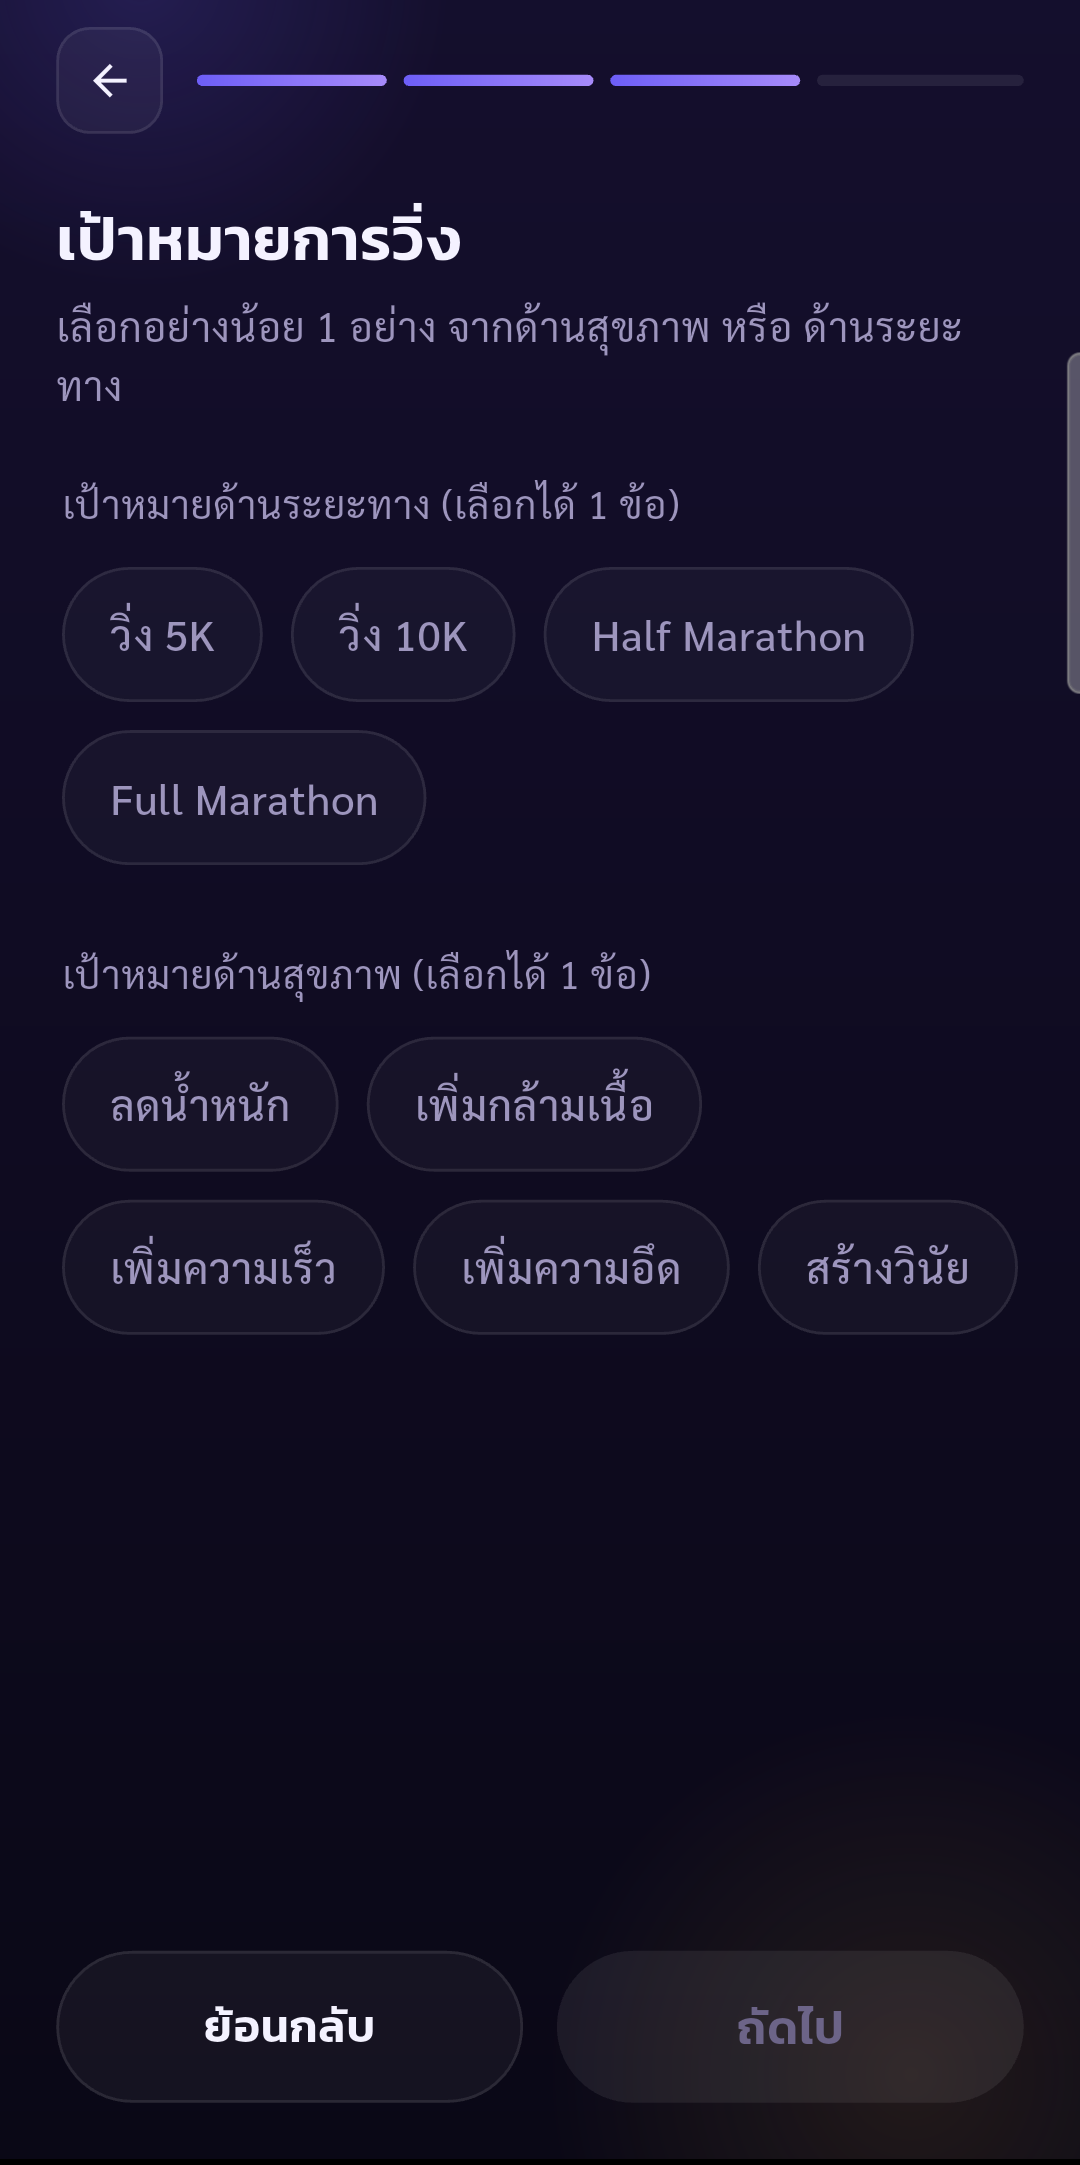
\includegraphics[width=\textwidth]{images/pegasus-onboarding-running-goals.png}\caption{เป้าหมายการวิ่ง}\end{subfigure}\hfill
\begin{subfigure}[t]{0.31\textwidth}\centering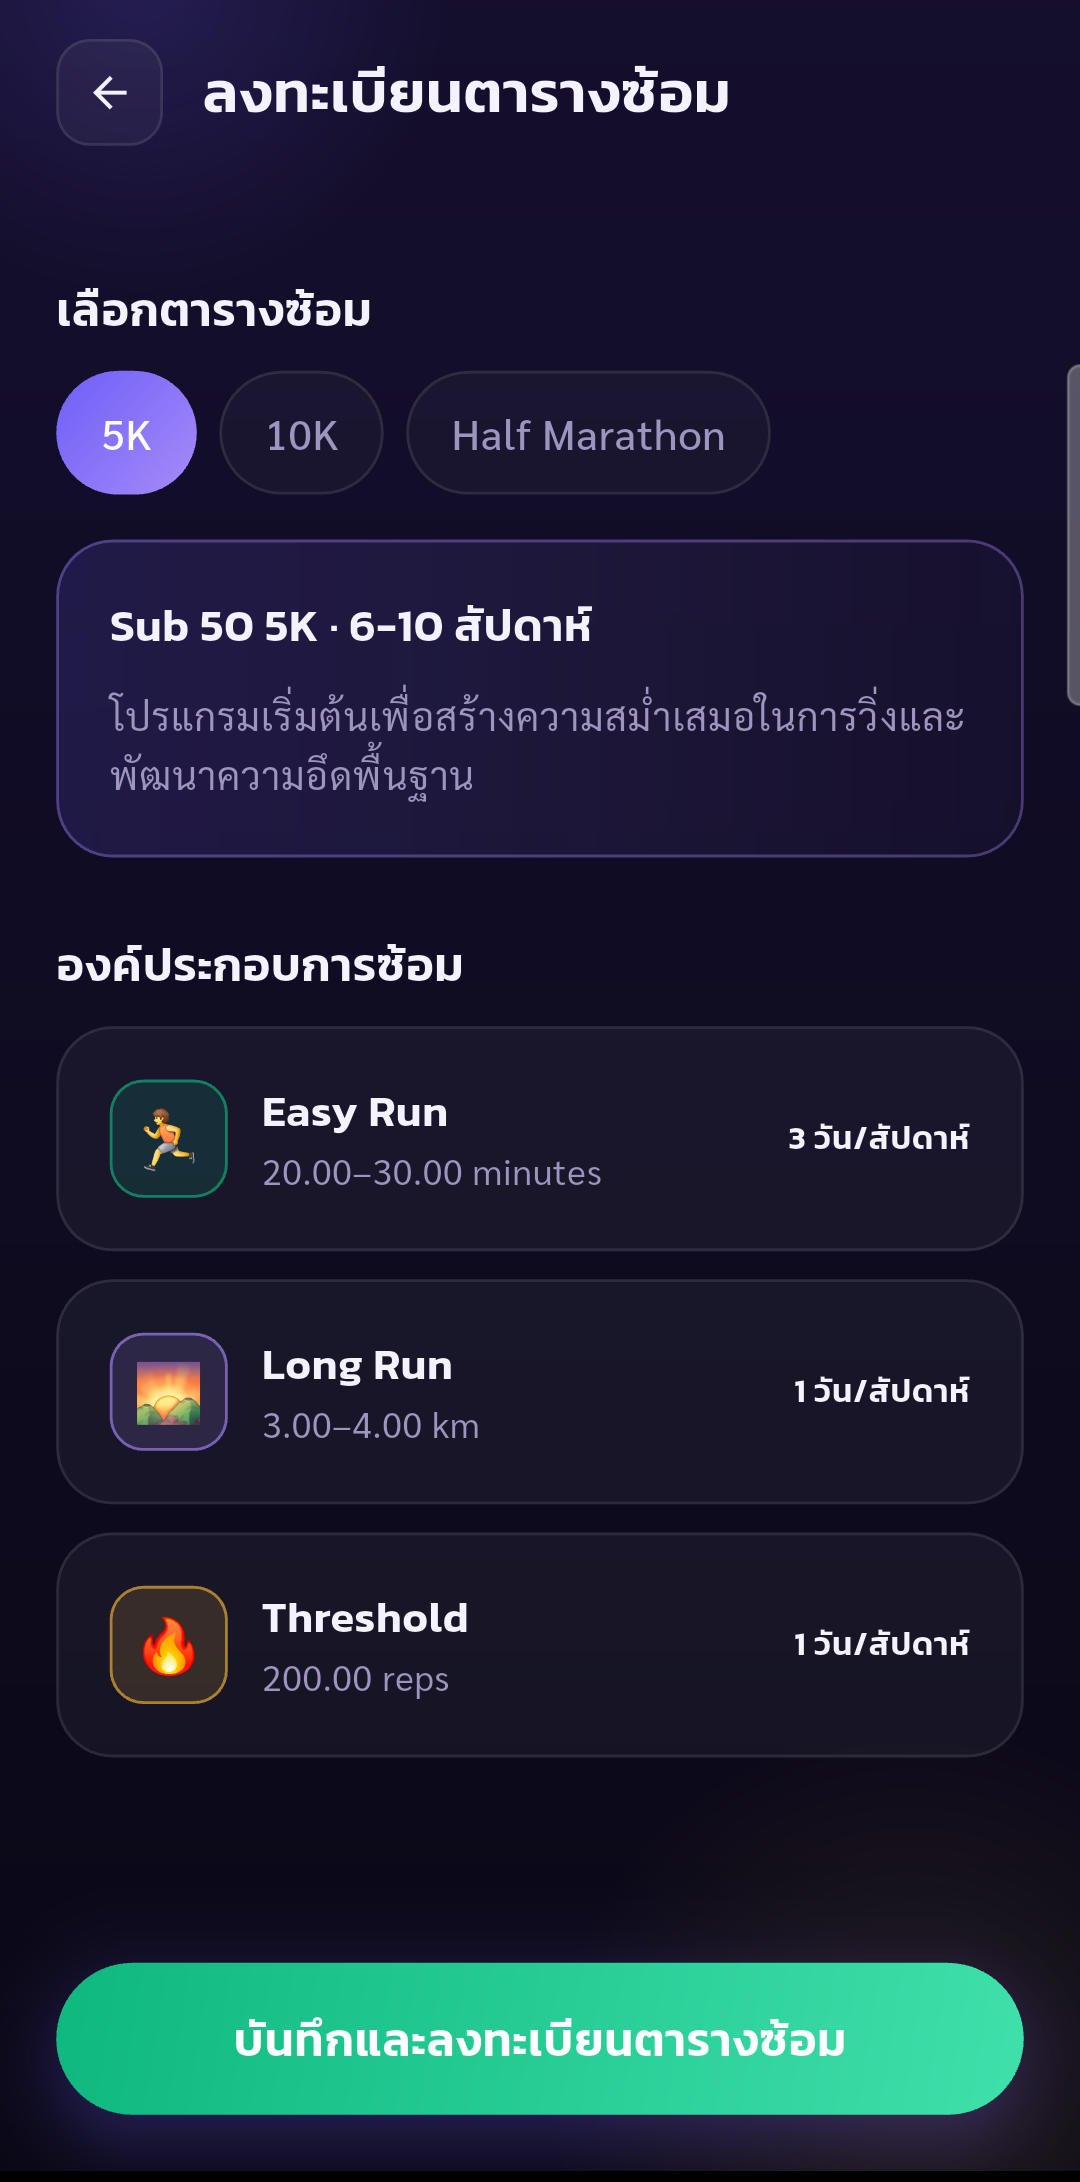
\includegraphics[width=\textwidth]{images/pegasus-training-plan-5k.png}\caption{แผน 5K}\end{subfigure}\hfill
\begin{subfigure}[t]{0.31\textwidth}\centering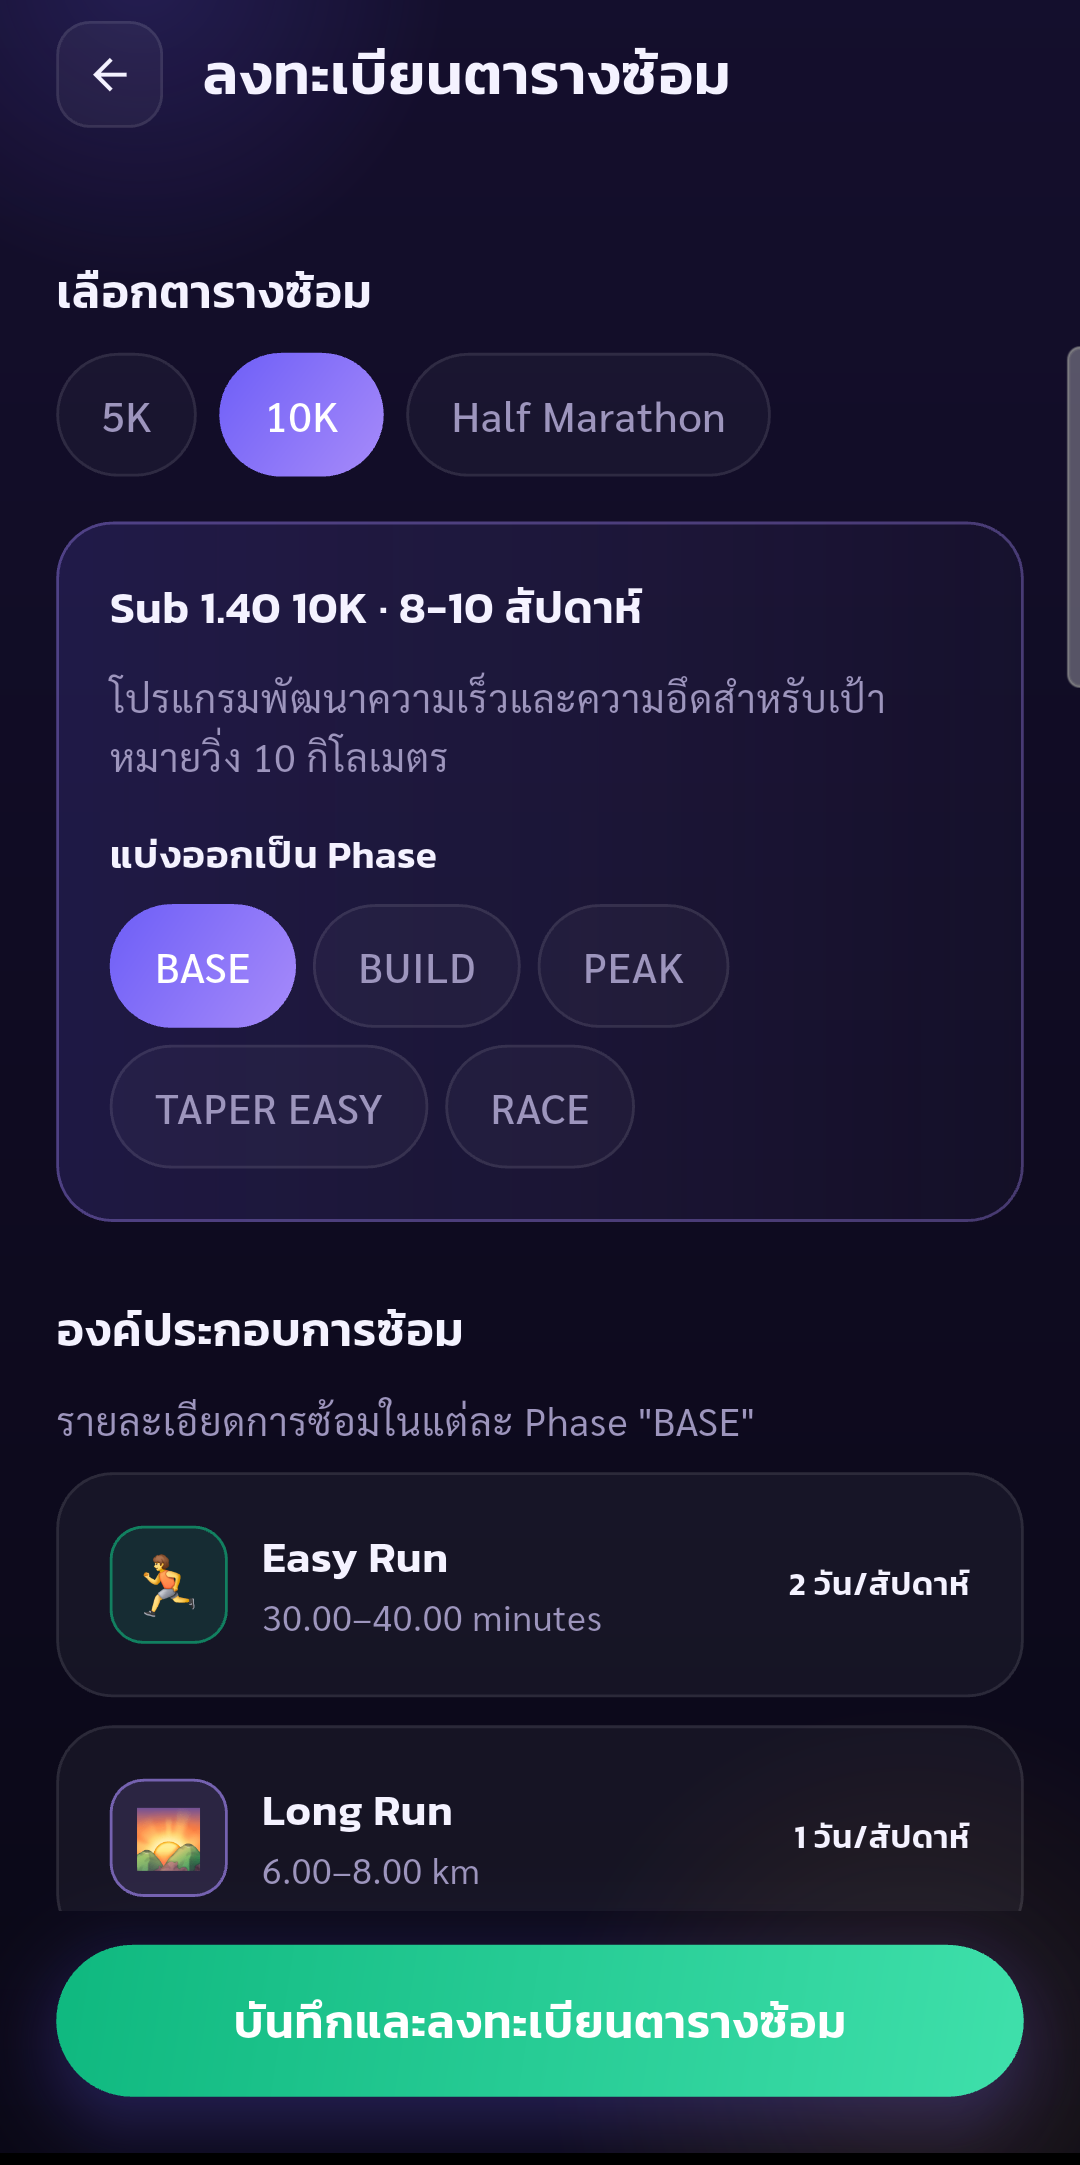
\includegraphics[width=\textwidth]{images/pegasus-training-plan-10k.png}\caption{แผน 10K}\end{subfigure}
\caption{การกำหนดเป้าหมายและการเลือกแผนการฝึก}\label{fig:app-goals}
\end{figure}

\begin{figure}[H]\centering
\begin{subfigure}[t]{0.31\textwidth}\centering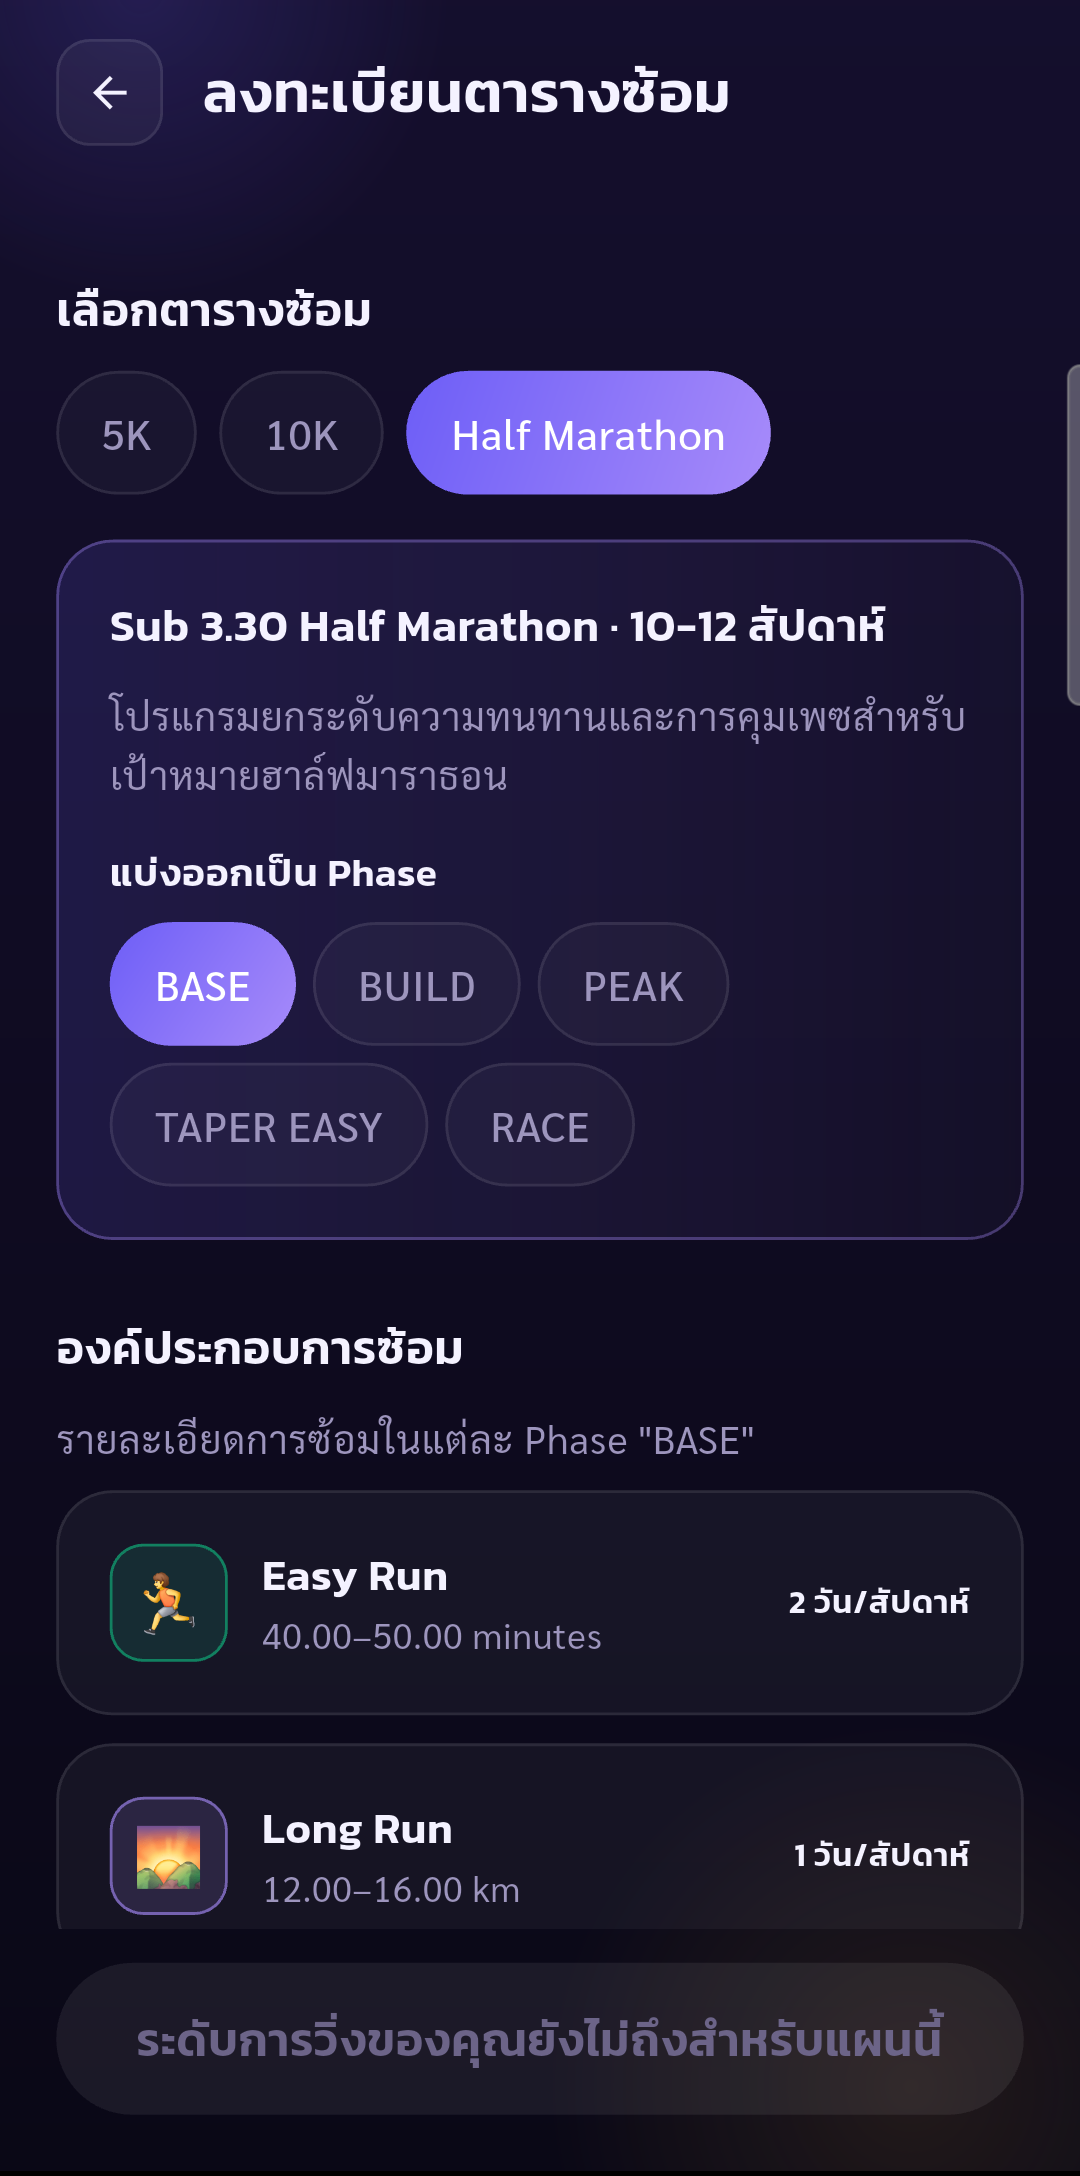
\includegraphics[width=\textwidth]{images/pegasus-training-plan-half-marathon.png}\caption{แผน Half Marathon}\end{subfigure}\hfill
\begin{subfigure}[t]{0.31\textwidth}\centering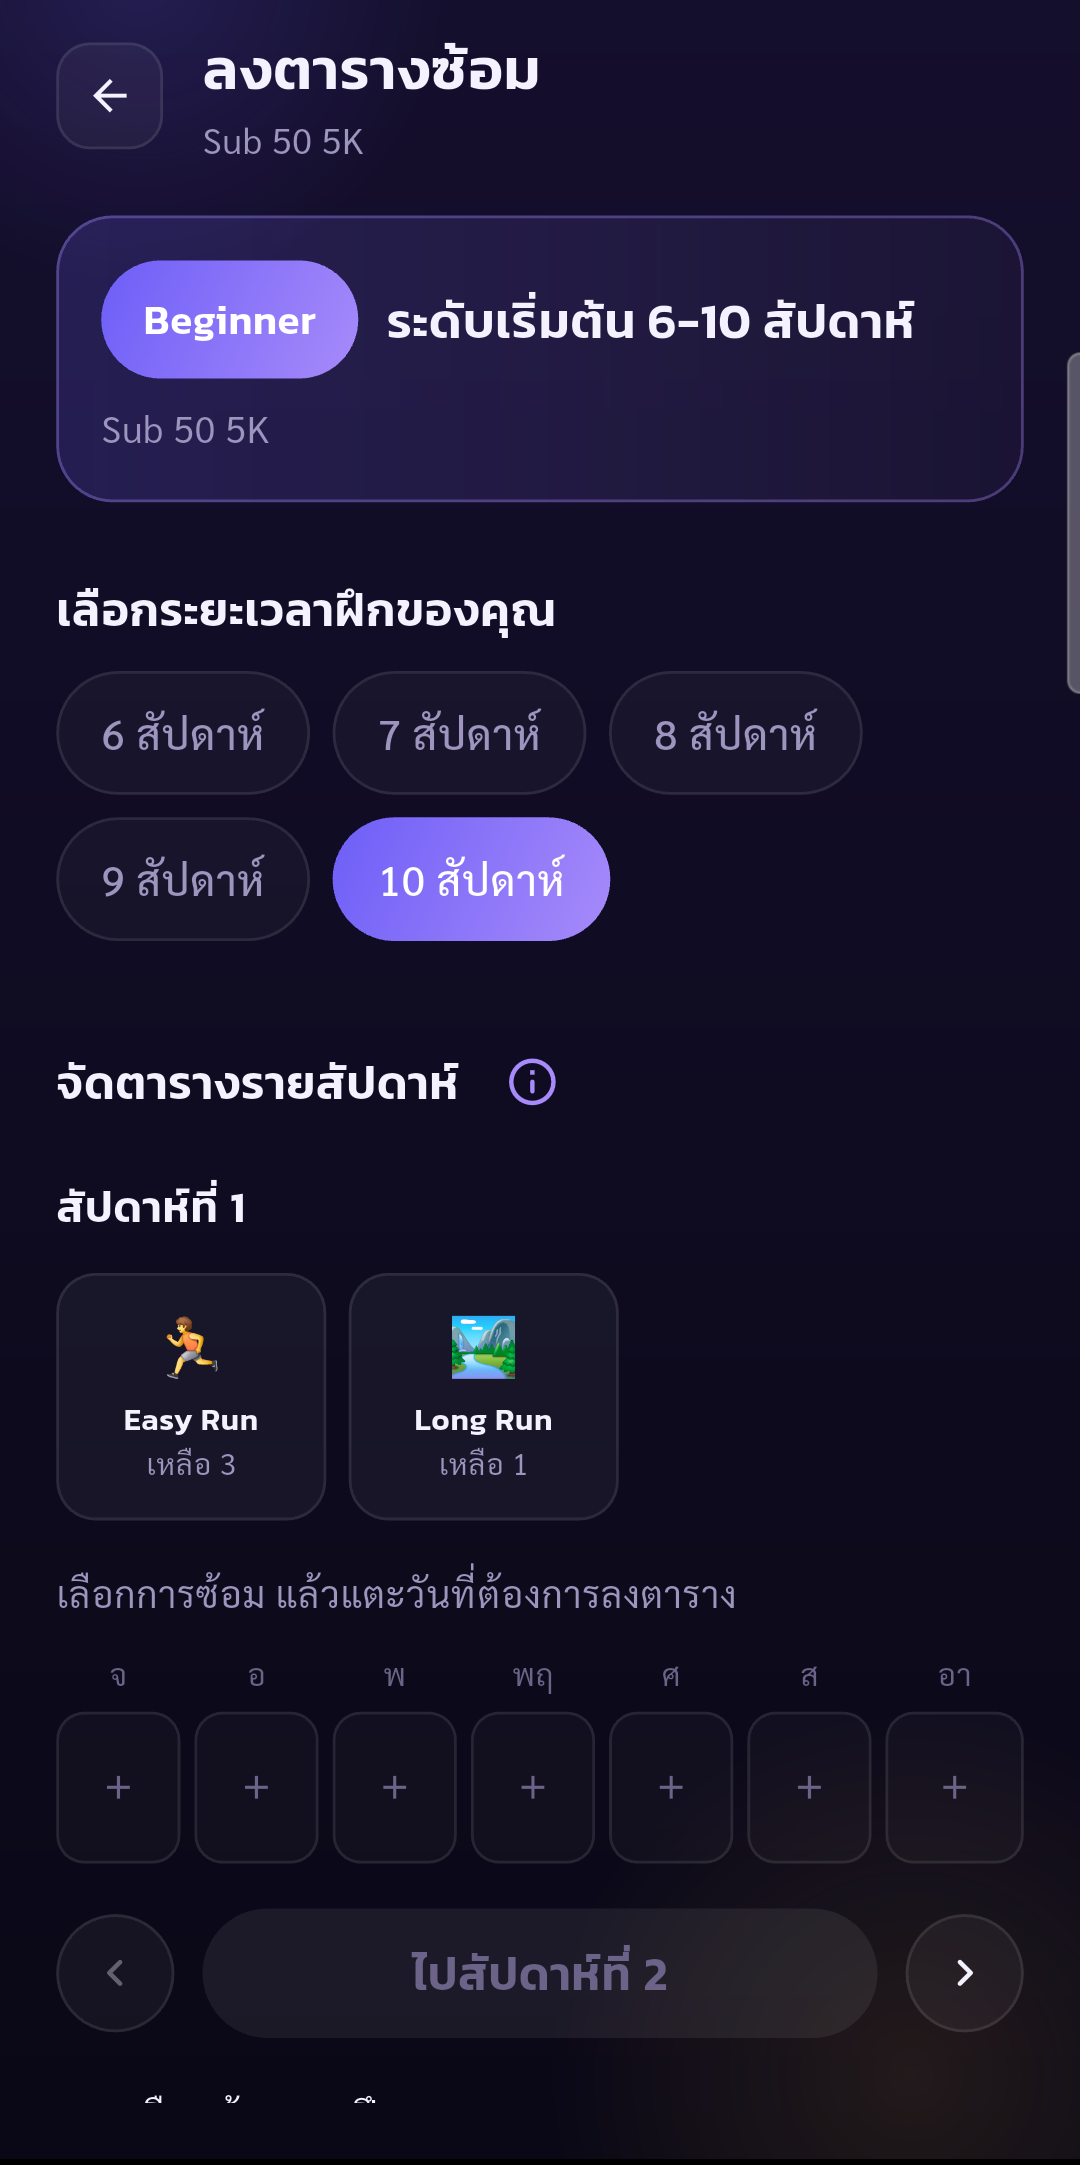
\includegraphics[width=\textwidth]{images/pegasus-schedule-builder-5k.png}\caption{จัดตารางแผน 5K}\end{subfigure}\hfill
\begin{subfigure}[t]{0.31\textwidth}\centering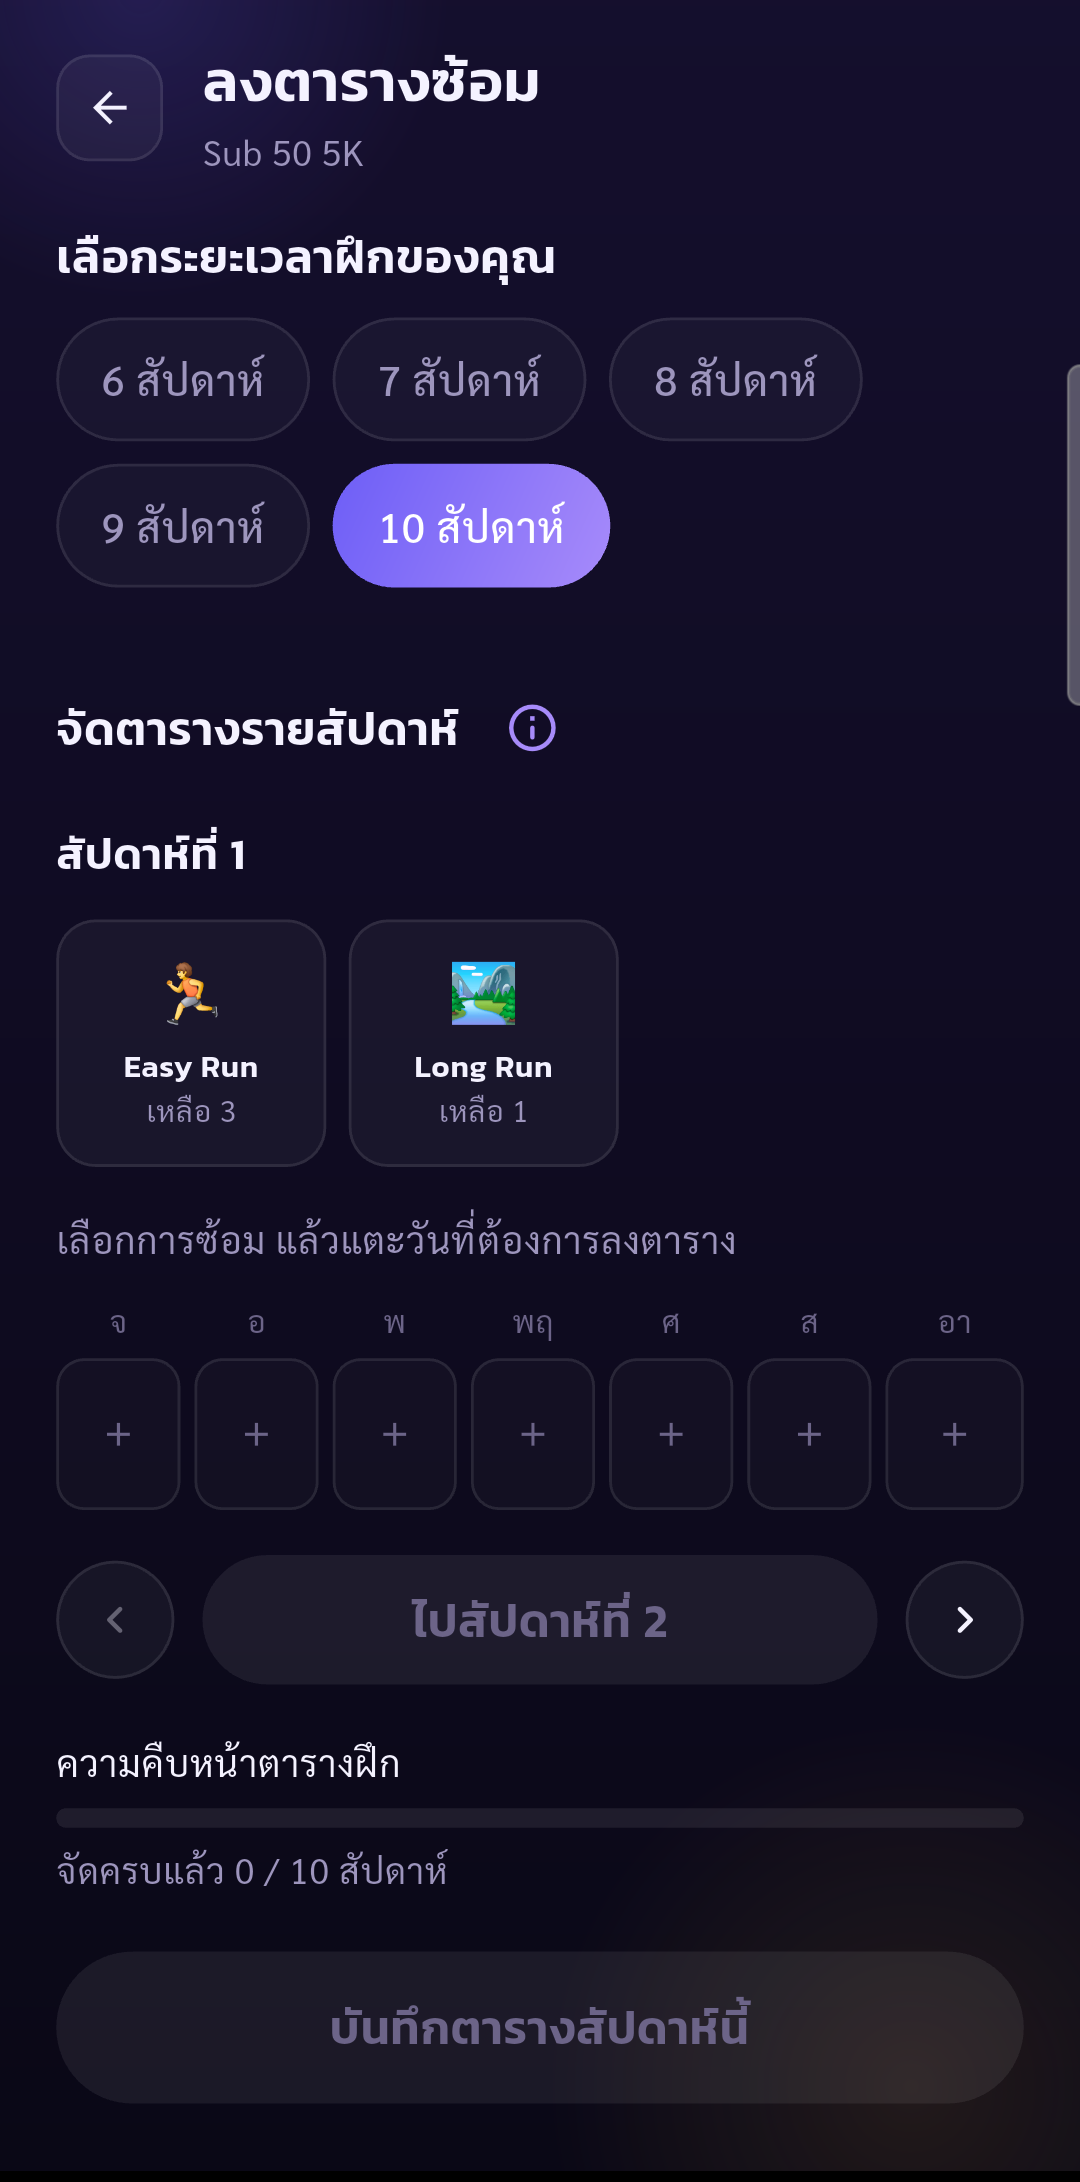
\includegraphics[width=\textwidth]{images/pegasus-schedule-builder-progress.png}\caption{ความคืบหน้าตารางฝึก}\end{subfigure}
\caption{รายละเอียดแผนการฝึกและการจัดตารางรายสัปดาห์}\label{fig:app-plans}
\end{figure}

\subsection*{หน้าหลักและ Daily Wellness Check-in}

หน้าหลักแสดงข้อมูลผู้ใช้ คะแนน เหรียญ กิจกรรมที่ต้องทำ Session การวิ่ง และแผนการฝึก ส่วน Daily Wellness Check-in ใช้ประเมินความพร้อมของผู้ใช้ในแต่ละวัน

\begin{figure}[H]\centering
\begin{subfigure}[t]{0.31\textwidth}\centering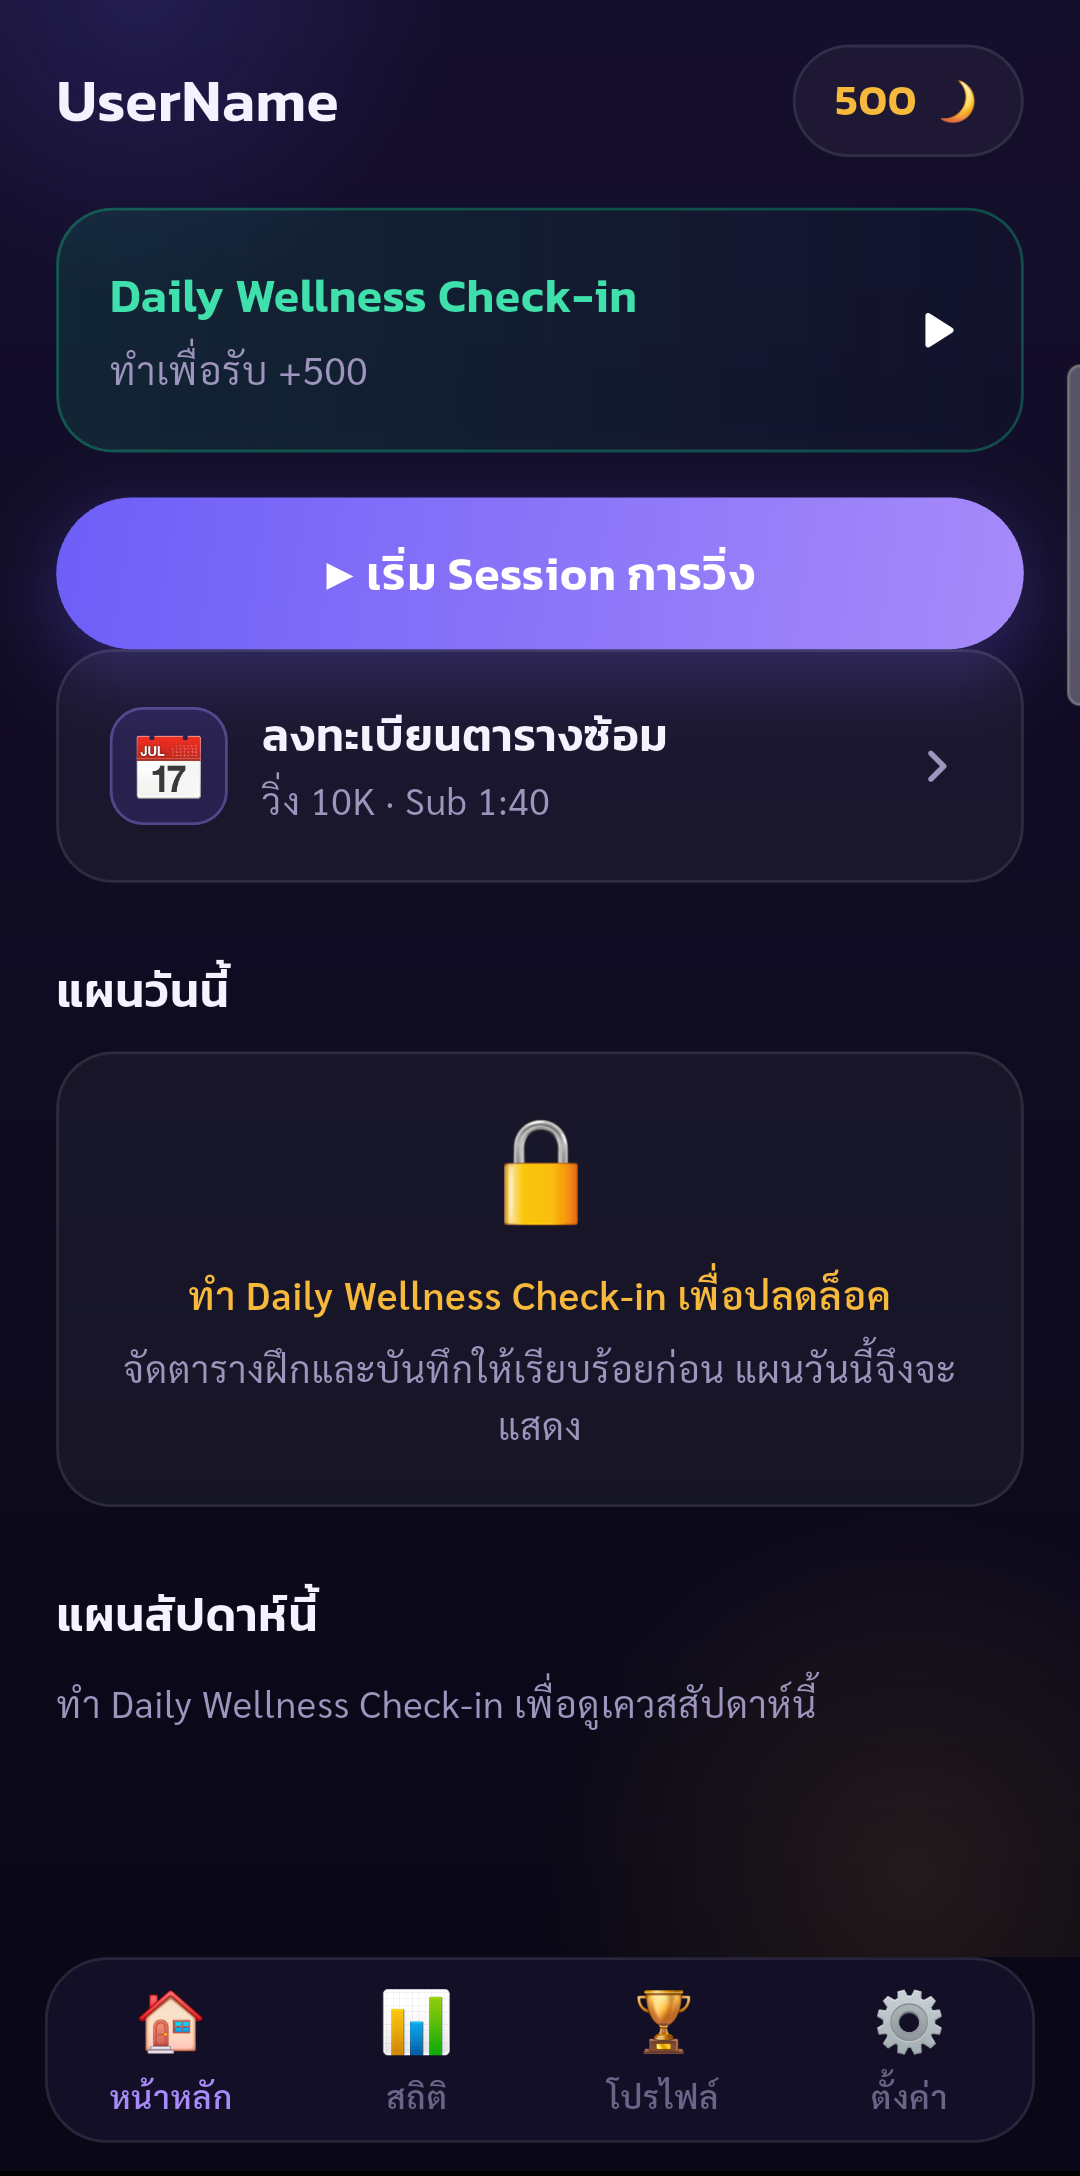
\includegraphics[width=\textwidth]{images/pegasus-home-locked.png}\caption{หน้าหลักก่อนปลดล็อก}\end{subfigure}\hfill
\begin{subfigure}[t]{0.31\textwidth}\centering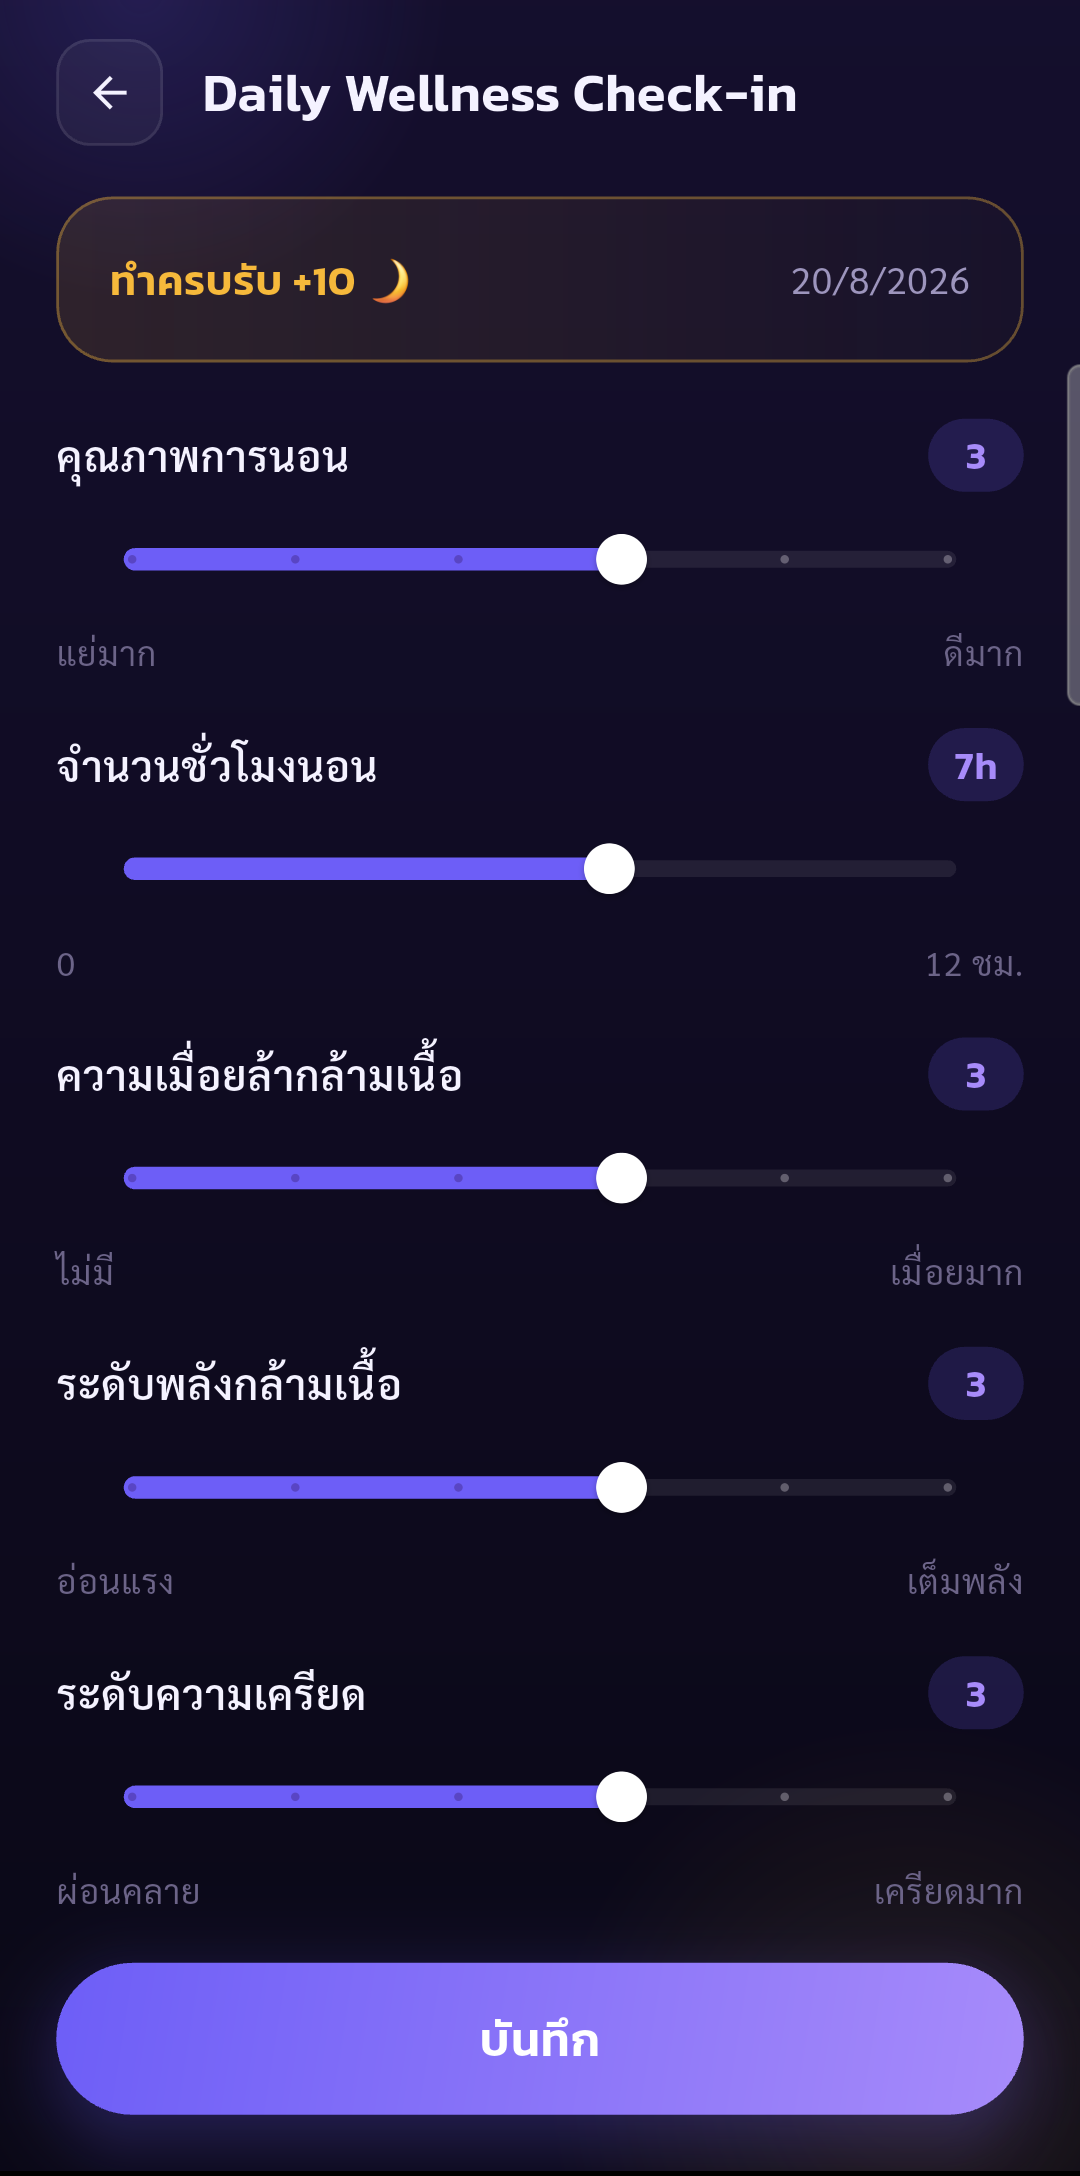
\includegraphics[width=\textwidth]{images/pegasus-daily-wellness-check-in.png}\caption{Daily Wellness Check-in}\end{subfigure}\hfill
\begin{subfigure}[t]{0.31\textwidth}\centering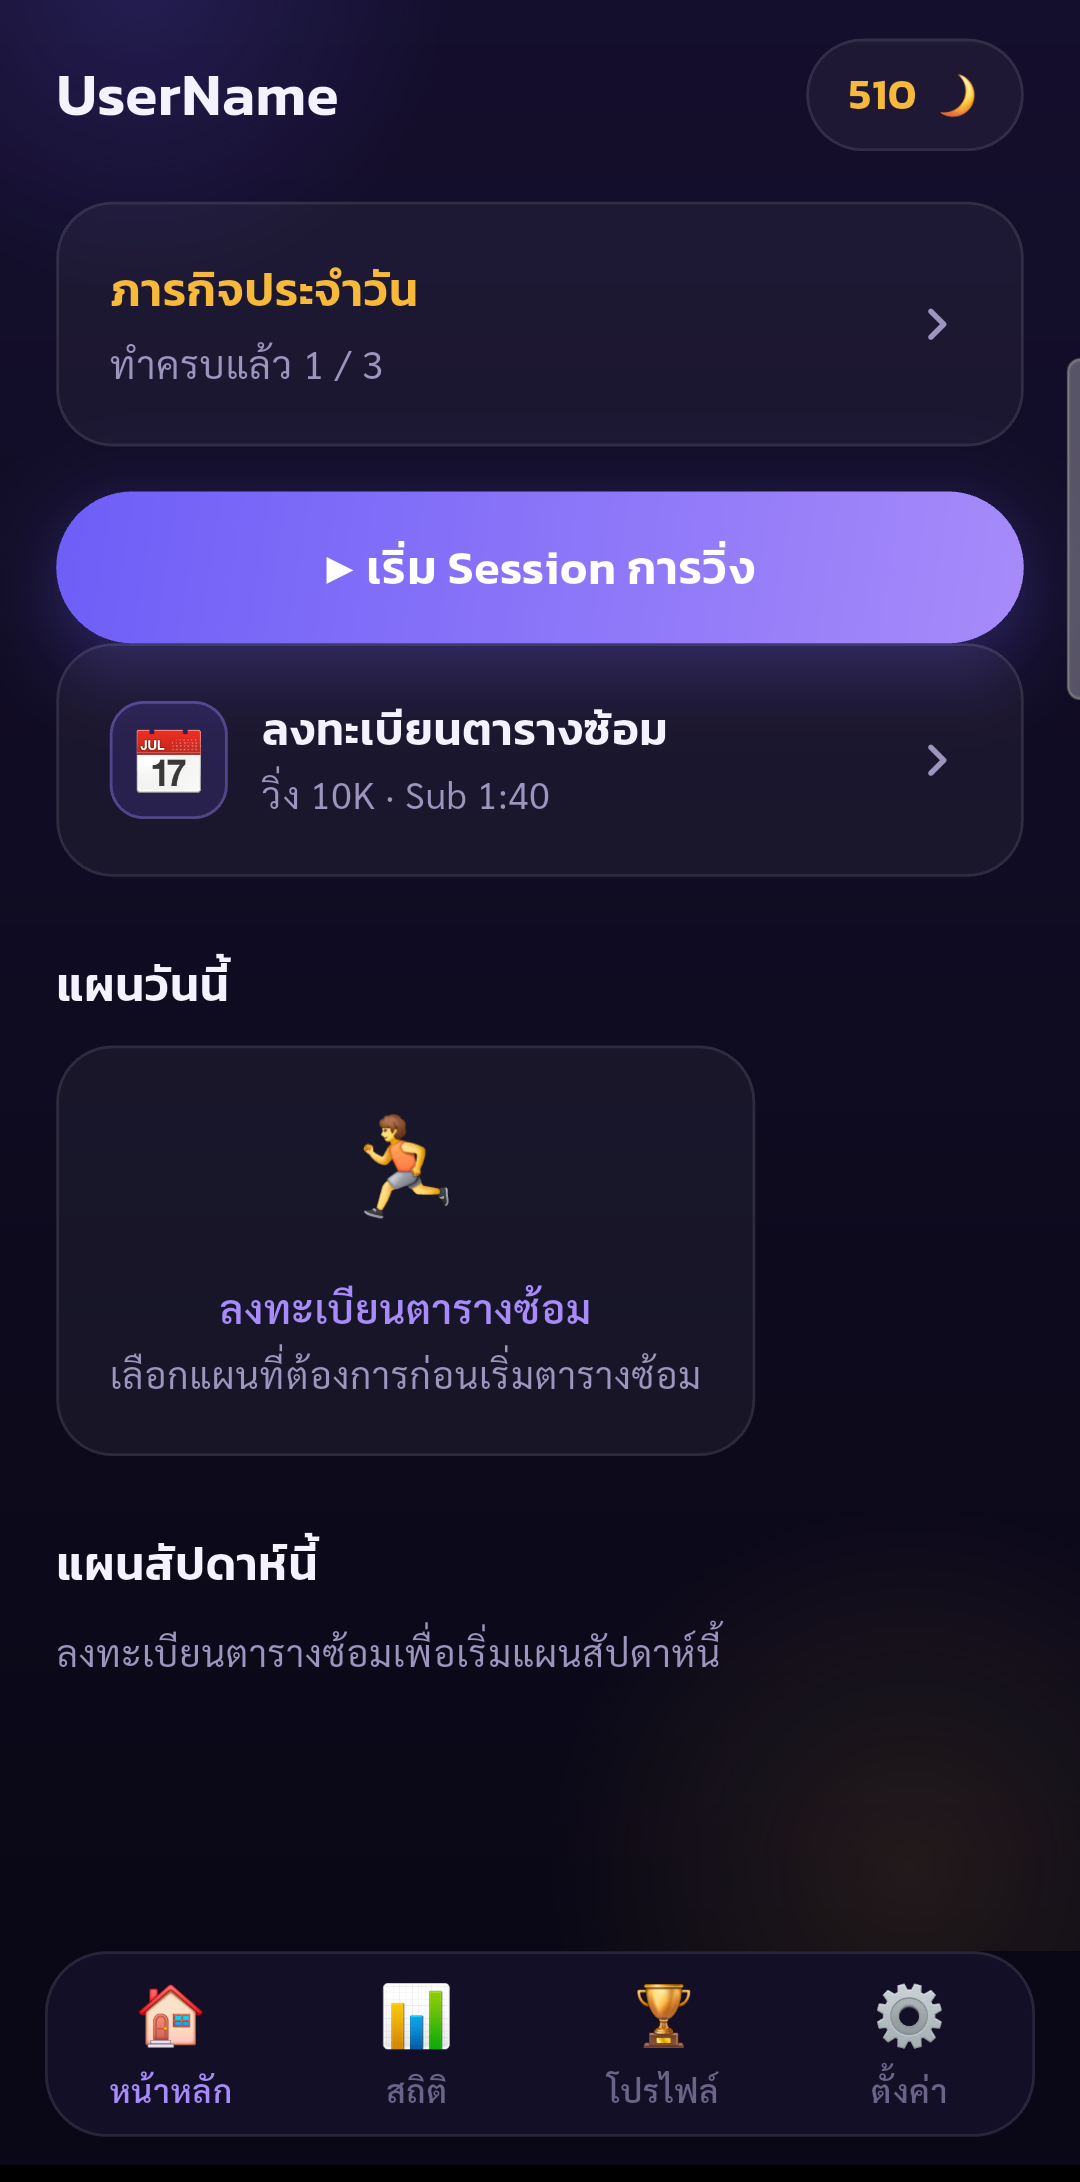
\includegraphics[width=\textwidth]{images/pegasus-home-training-required.png}\caption{หน้าหลักหลังการเช็กอิน}\end{subfigure}
\caption{หน้าหลักและการประเมินความพร้อมประจำวัน}\label{fig:app-home-wellness}
\end{figure}

\begin{figure}[H]\centering
\begin{subfigure}[t]{0.31\textwidth}\centering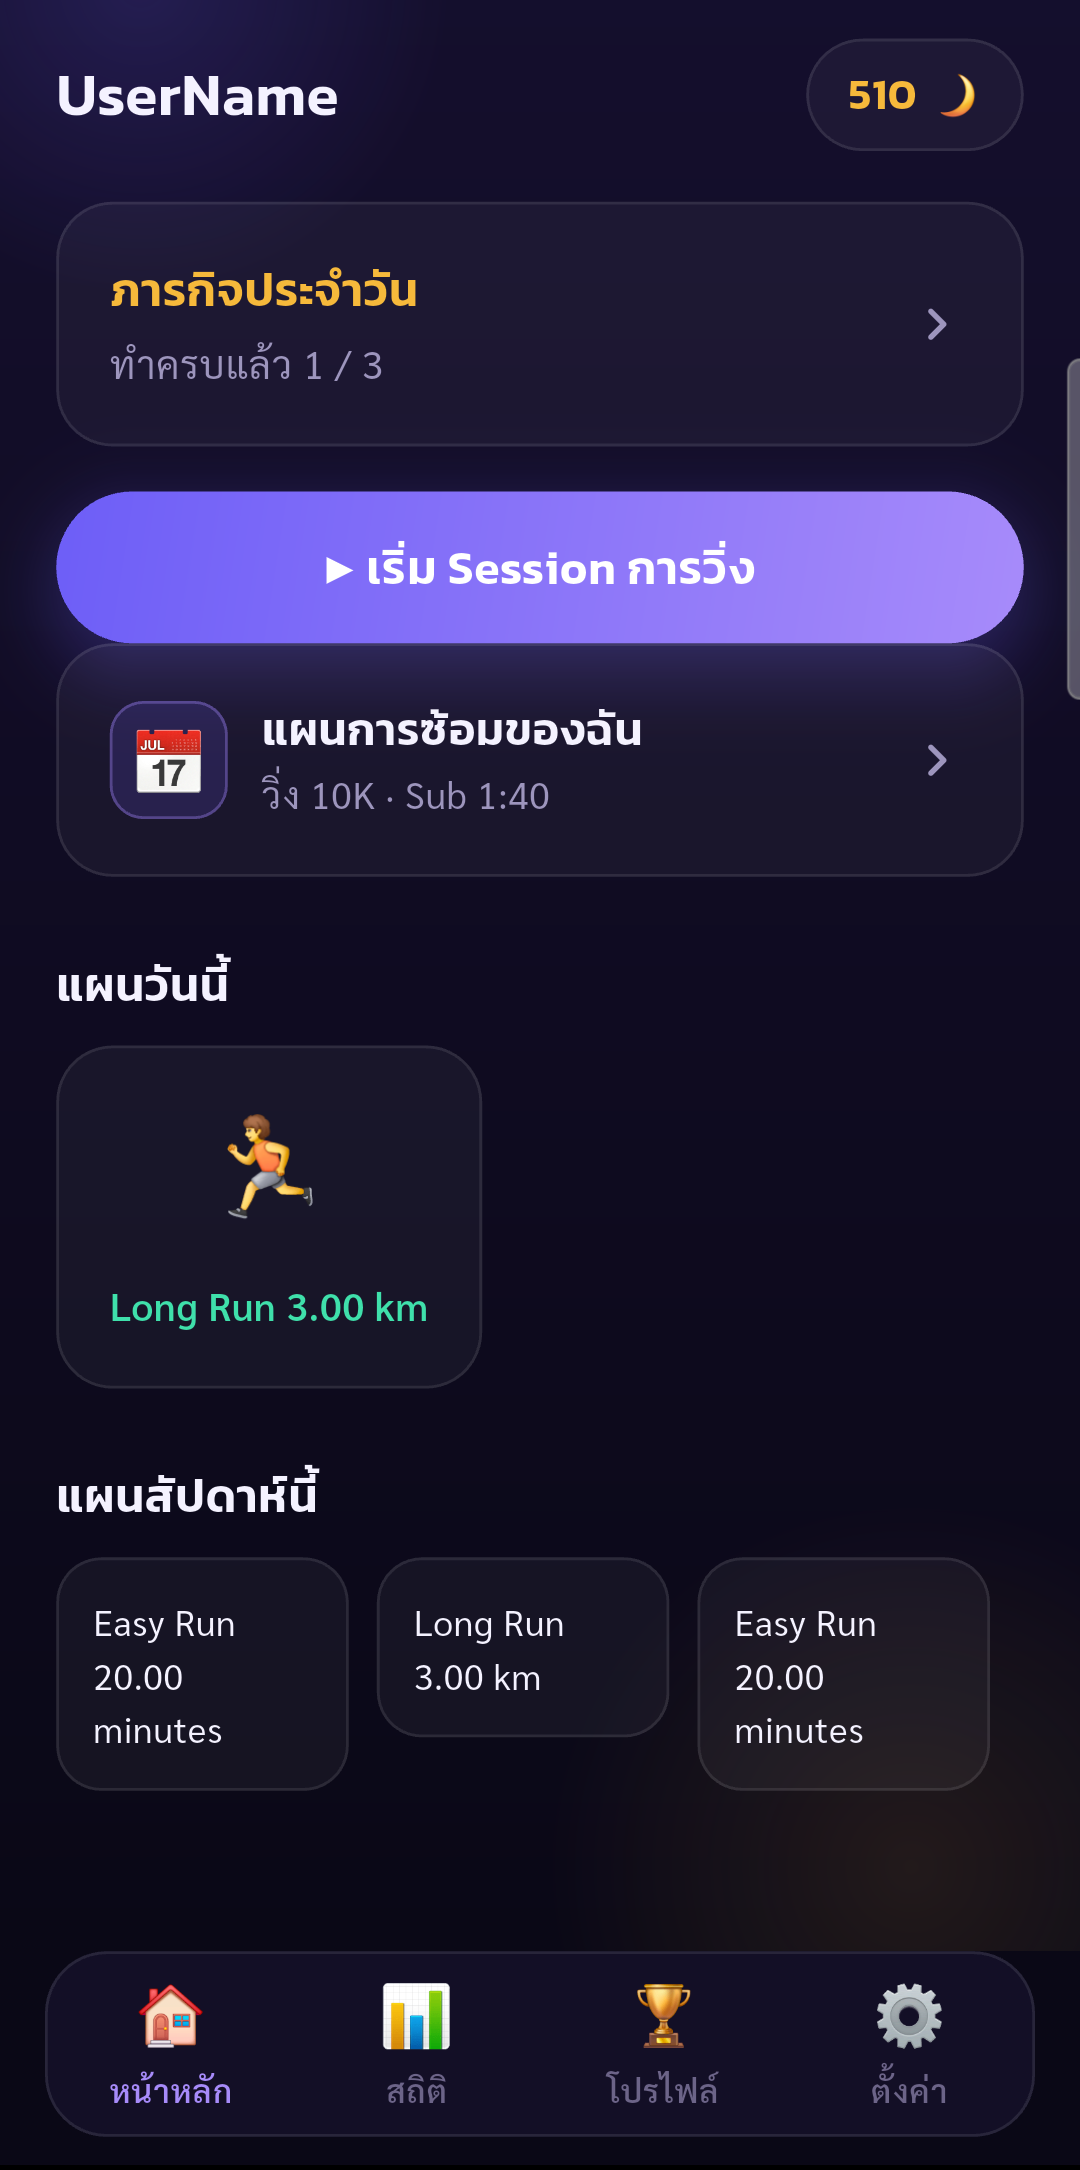
\includegraphics[width=\textwidth]{images/pegasus-home-training-scheduled.png}\caption{หน้าหลักพร้อมแผนฝึก}\end{subfigure}\hfill
\begin{subfigure}[t]{0.31\textwidth}\centering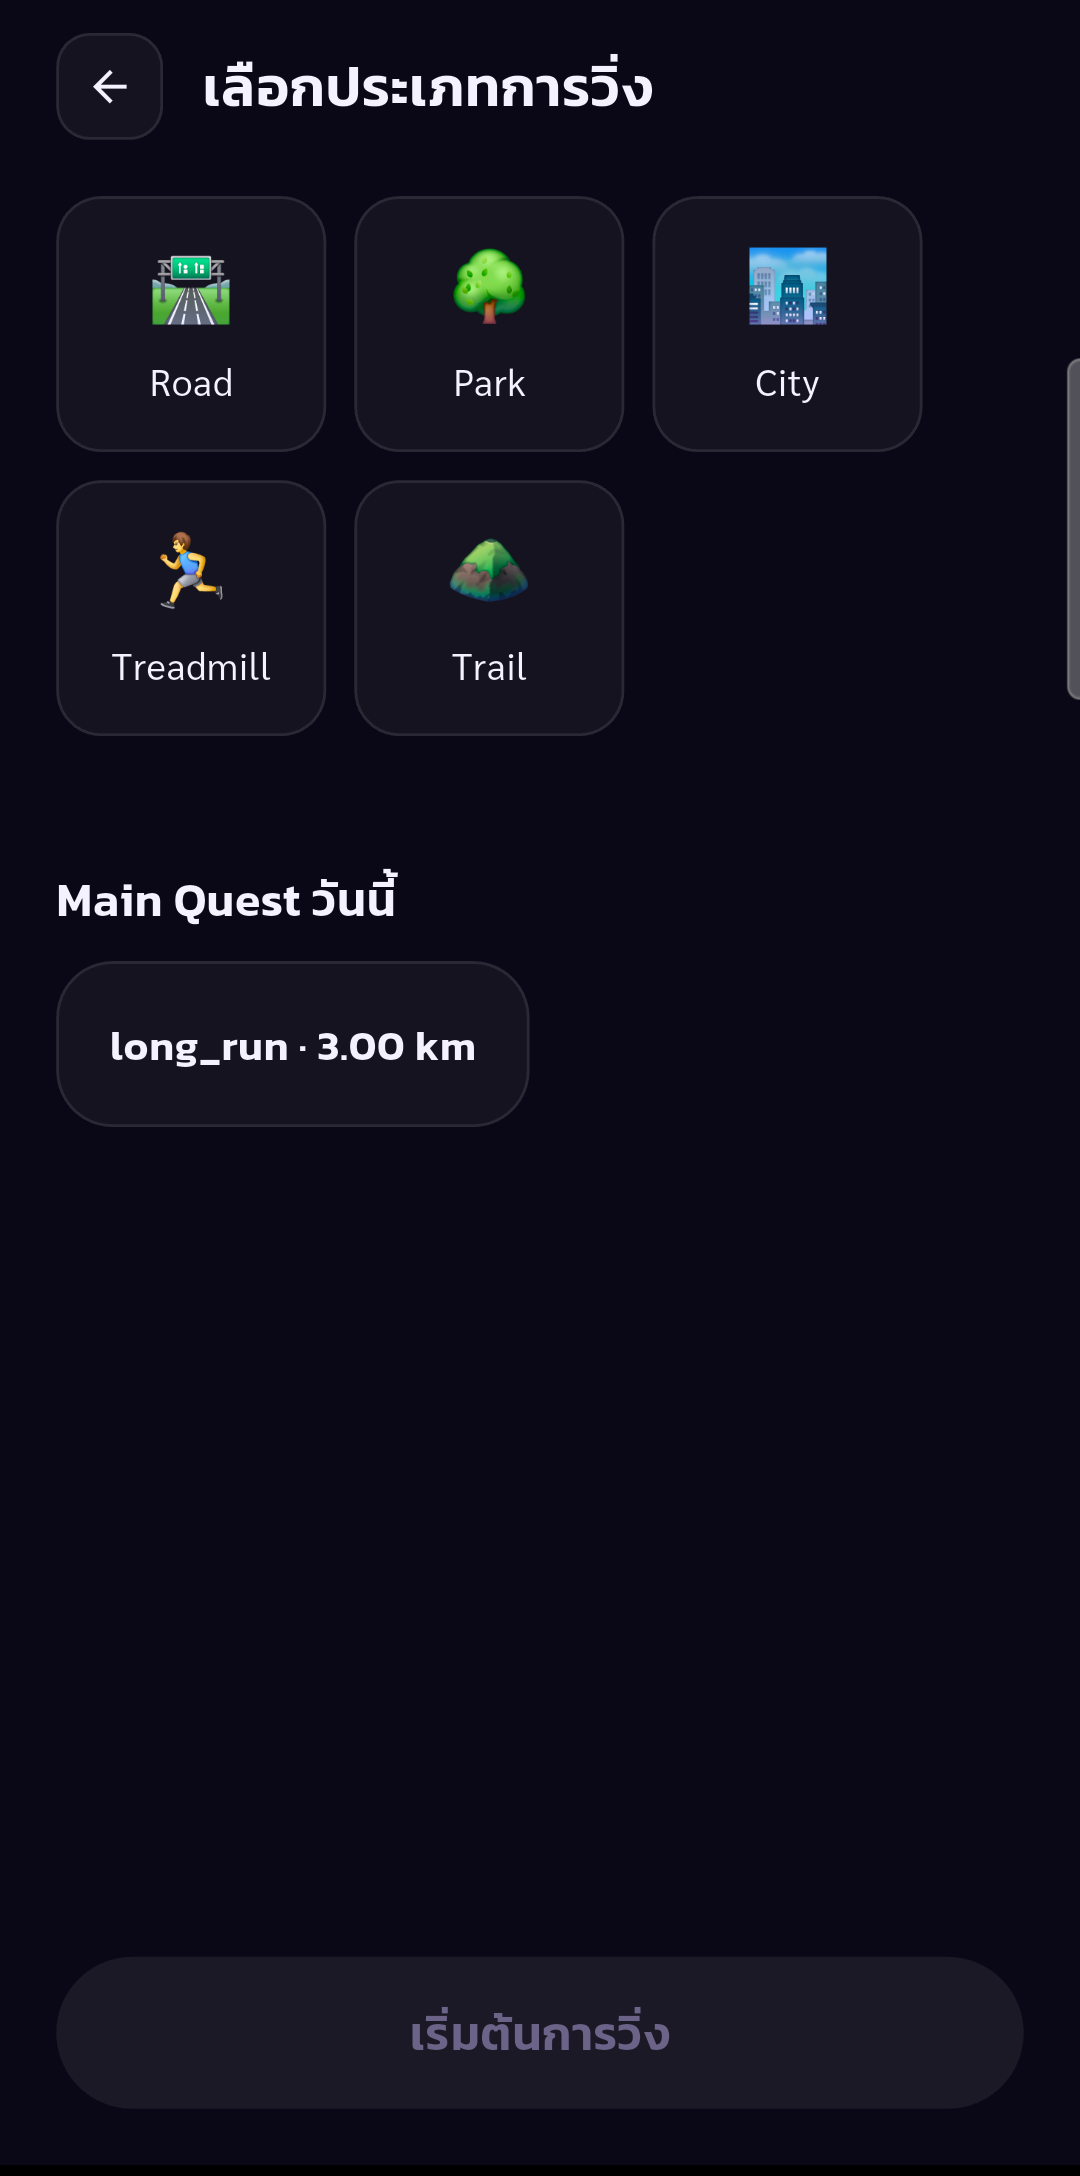
\includegraphics[width=\textwidth]{images/pegasus-run-session-type-selection.png}\caption{เลือกประเภทการวิ่ง}\end{subfigure}\hfill
\begin{subfigure}[t]{0.31\textwidth}\centering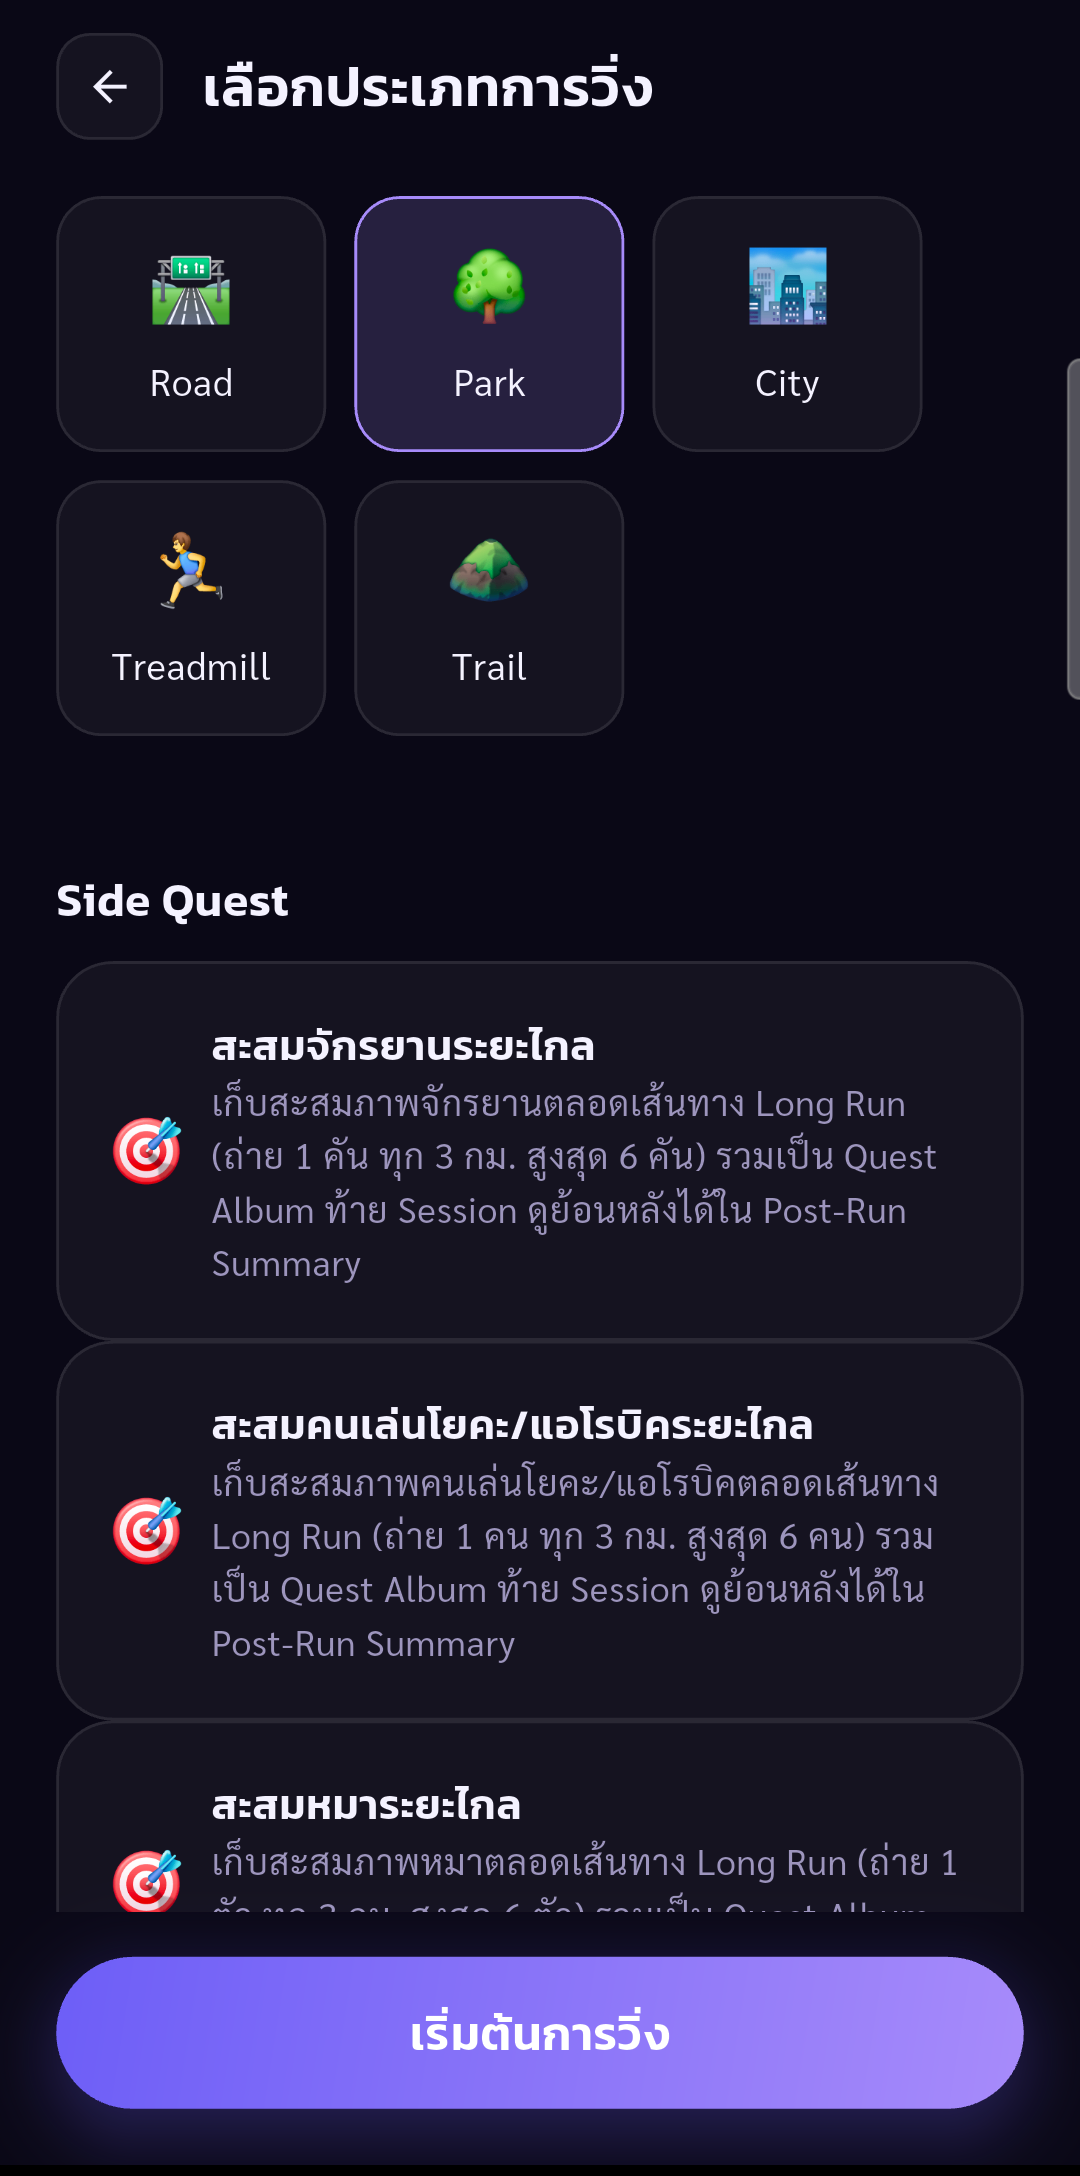
\includegraphics[width=\textwidth]{images/pegasus-run-session-quests.png}\caption{ภารกิจระหว่างการวิ่ง}\end{subfigure}
\caption{หน้าหลักและการเตรียมเริ่ม Session การวิ่ง}\label{fig:app-session-preparation}
\end{figure}

\subsection*{การวิ่งและผลลัพธ์หลังวิ่ง}

หน้าจอ Active Run Session แสดงเวลา ระยะทาง Pace ตำแหน่งบนแผนที่ และภารกิจที่กำลังดำเนินการ เมื่อจบการวิ่ง ระบบจะแสดงหน้าสรุปผลเพื่อให้ผู้ใช้ประเมิน RPE ระดับความเครียด และความรู้สึกหลังวิ่ง

\begin{figure}[H]\centering
\begin{subfigure}[t]{0.31\textwidth}\centering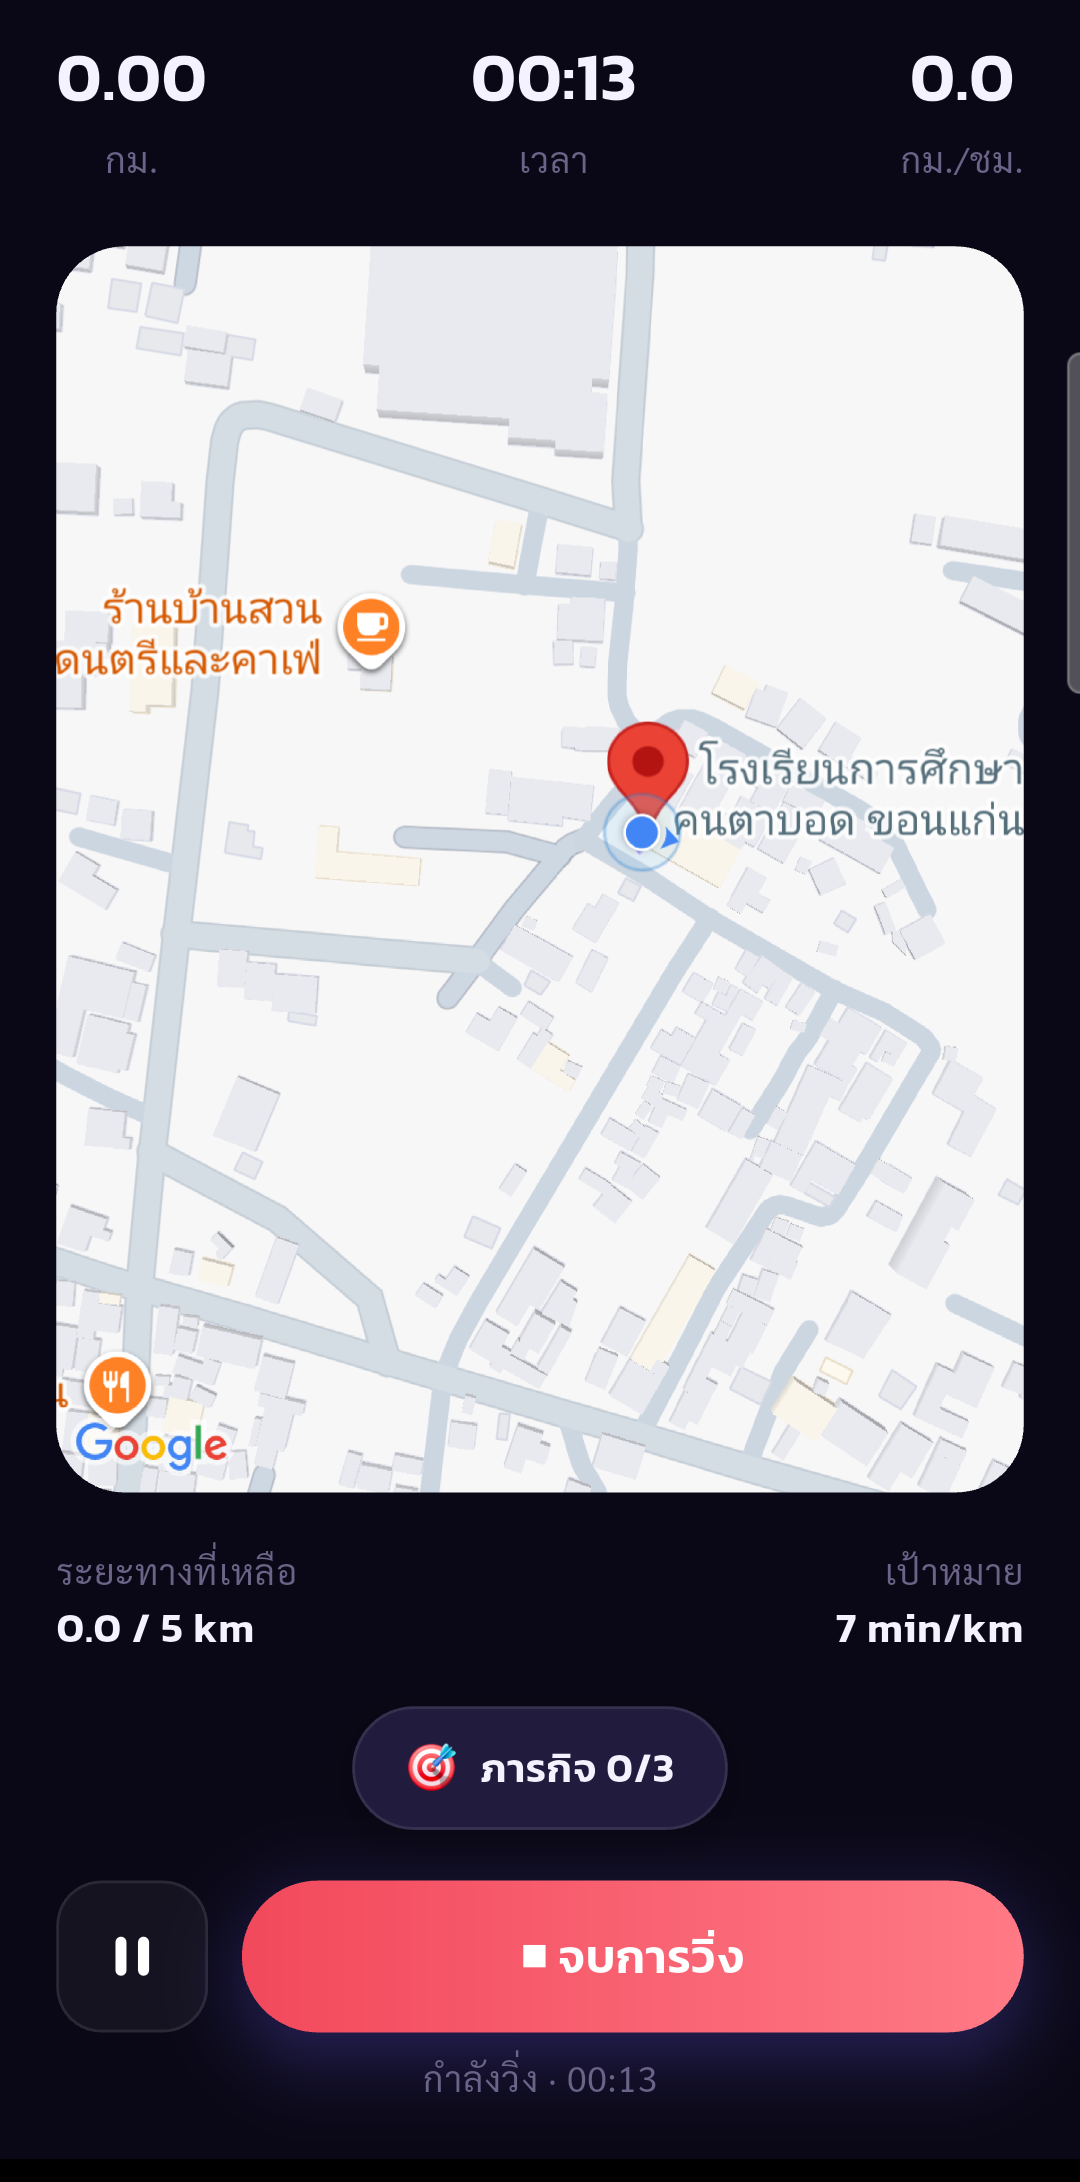
\includegraphics[width=\textwidth]{images/pegasus-active-run-session.png}\caption{กำลังวิ่ง}\end{subfigure}\hfill
\begin{subfigure}[t]{0.31\textwidth}\centering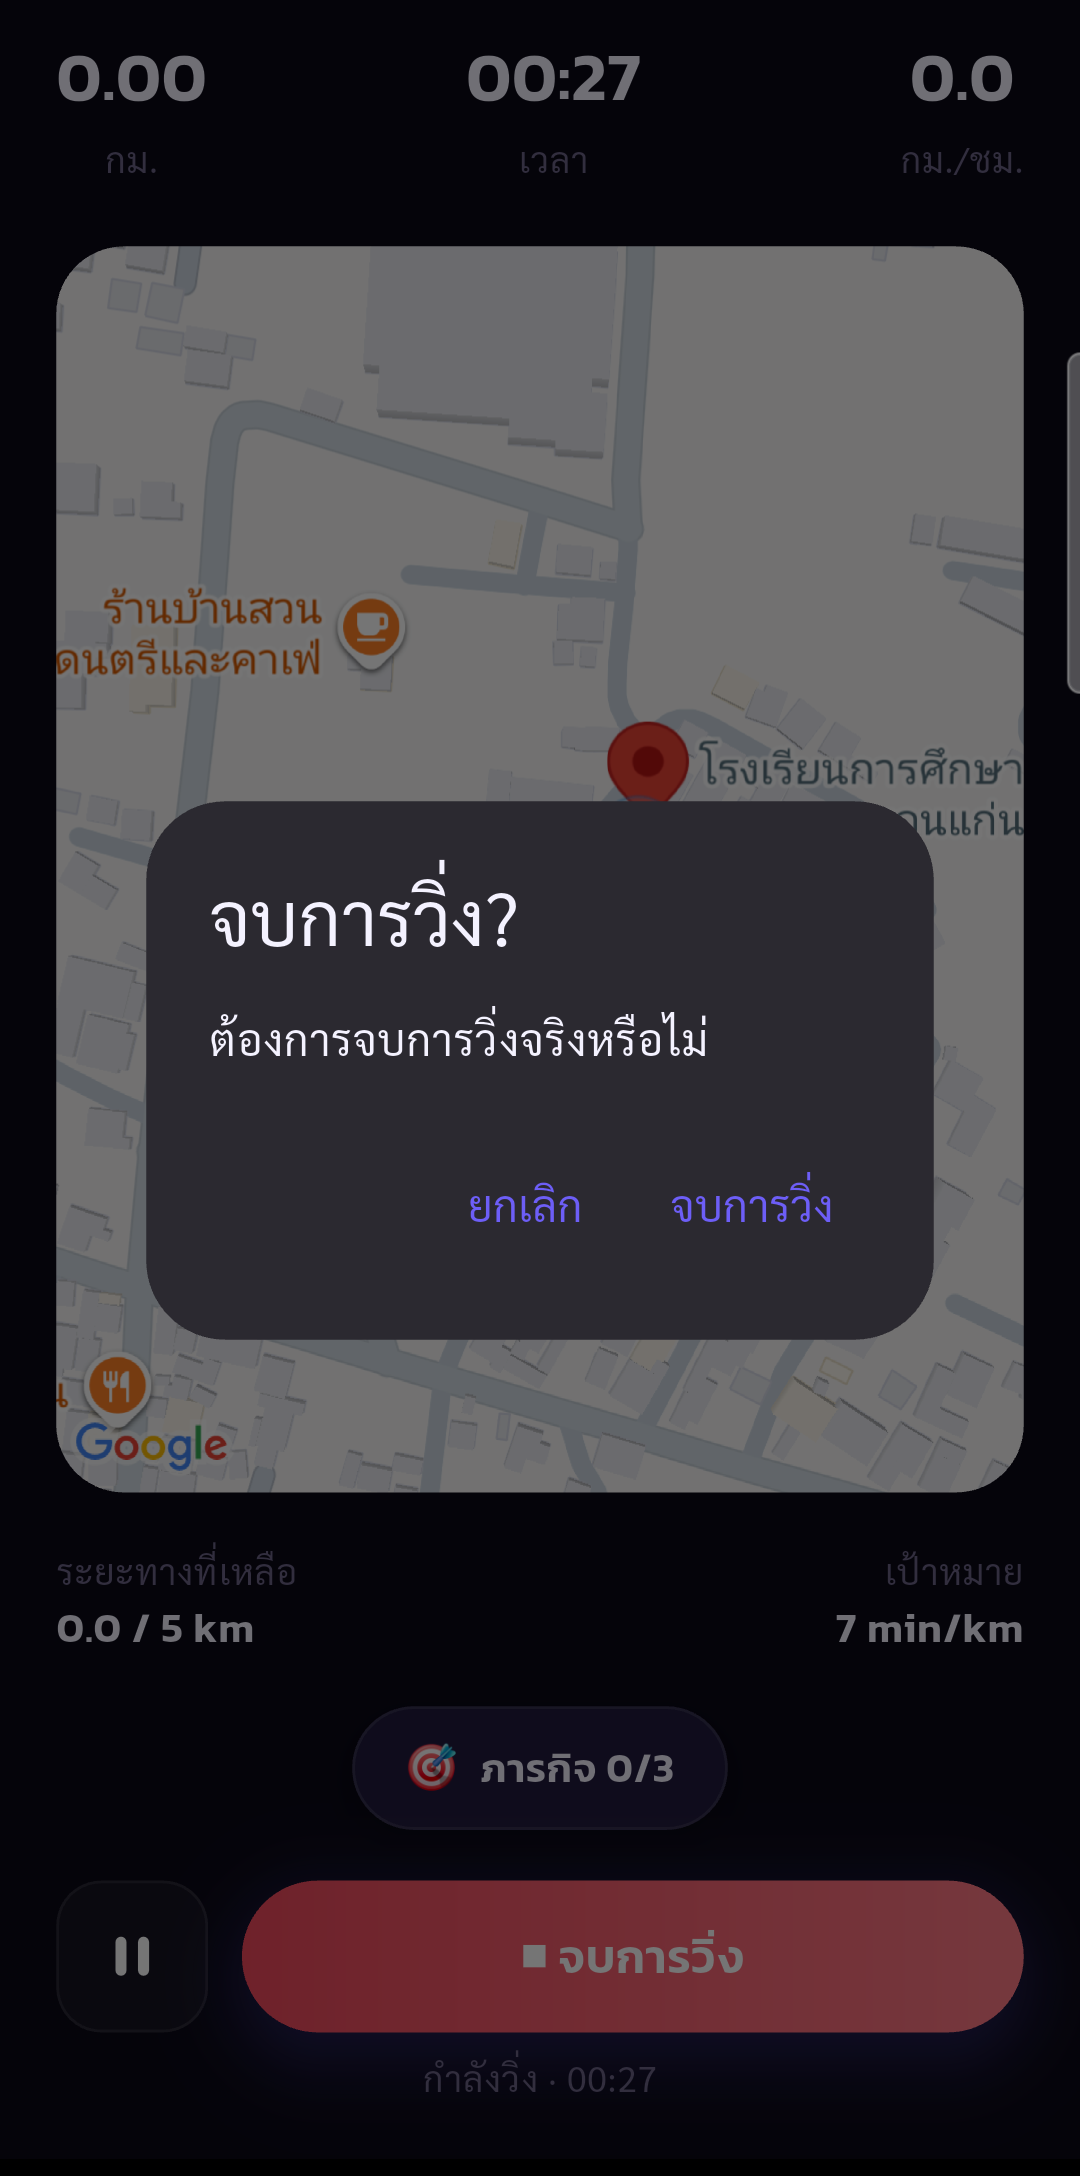
\includegraphics[width=\textwidth]{images/pegasus-end-run-confirmation.png}\caption{ยืนยันจบการวิ่ง}\end{subfigure}\hfill
\begin{subfigure}[t]{0.31\textwidth}\centering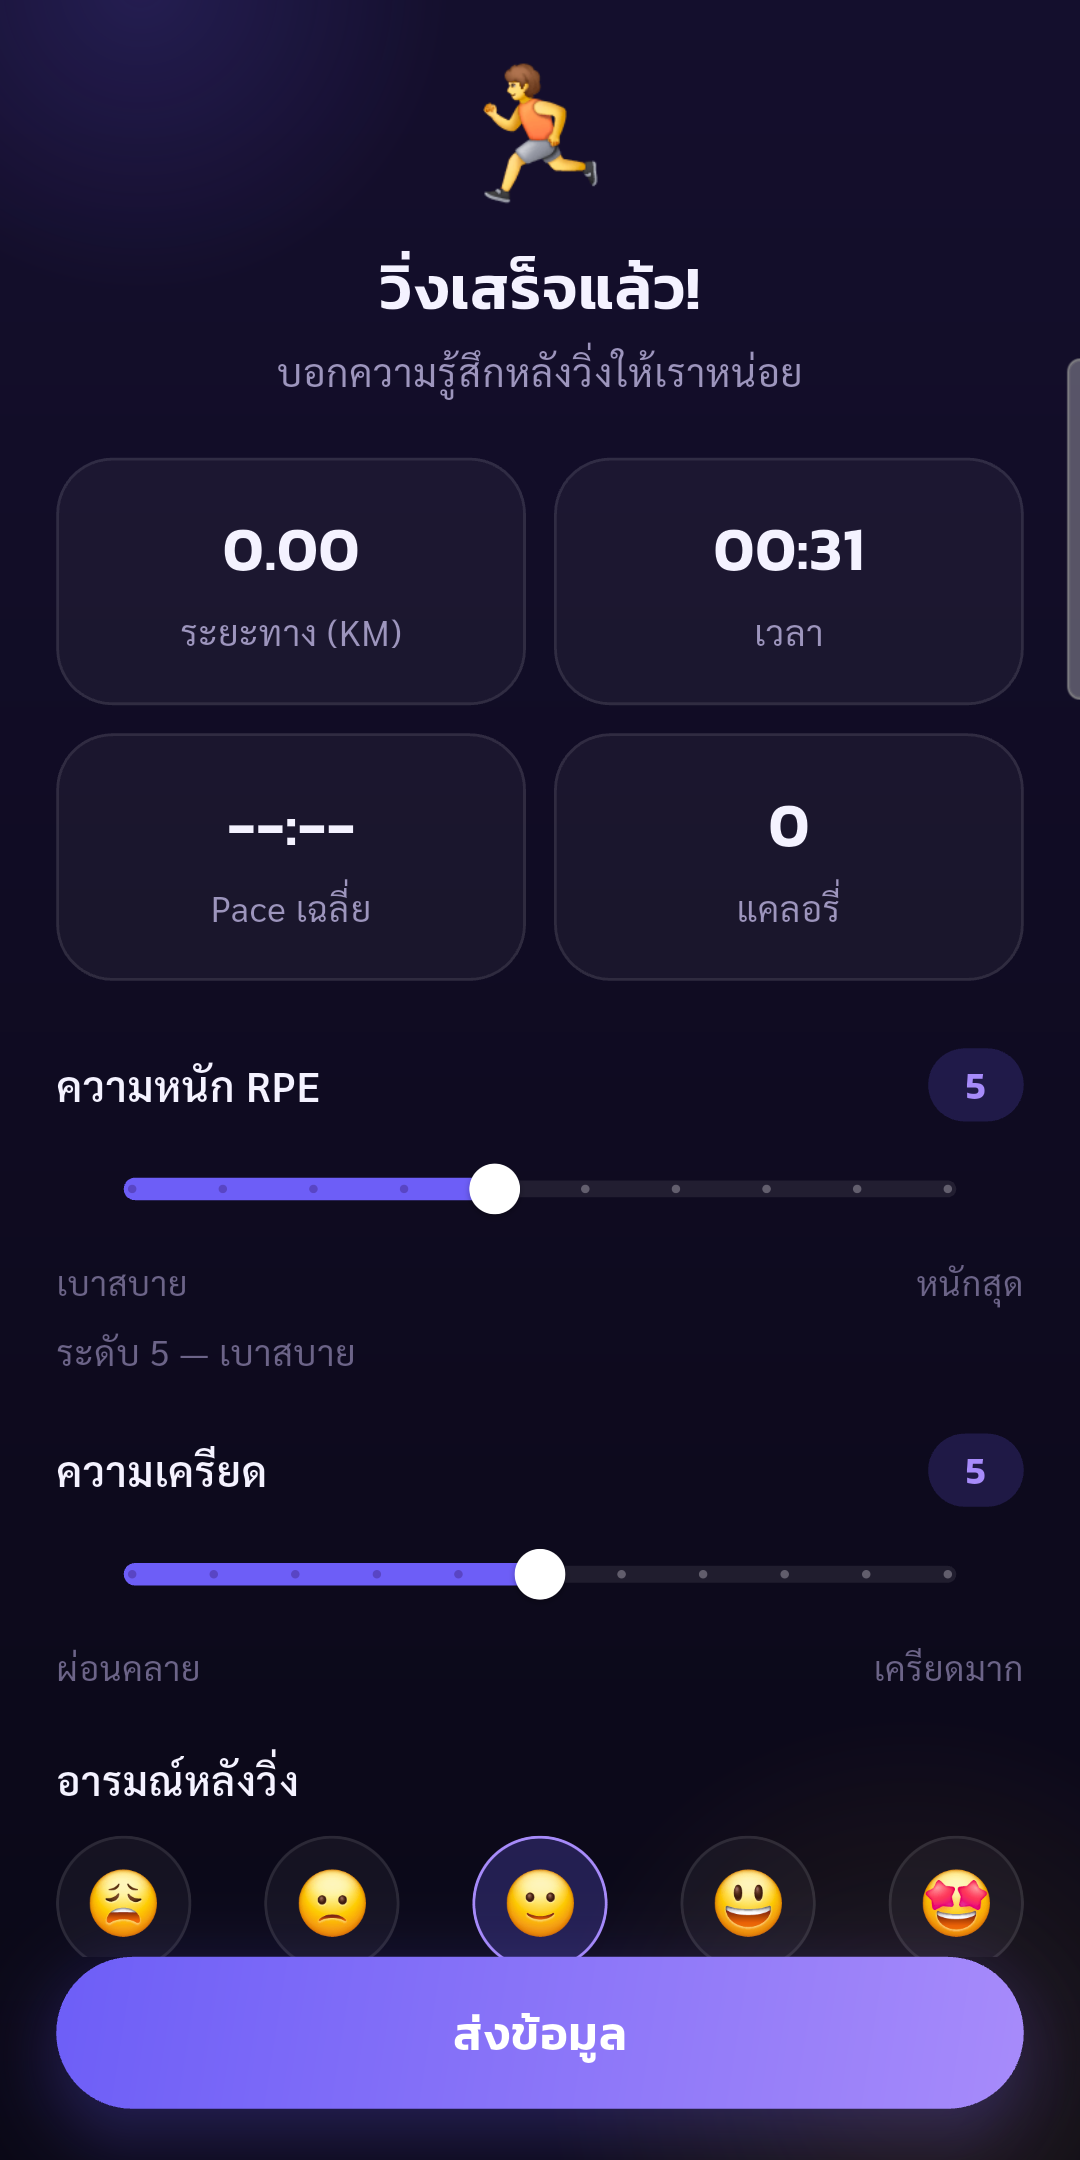
\includegraphics[width=\textwidth]{images/pegasus-post-run-feedback.png}\caption{สรุปผลและ Feedback}\end{subfigure}
\caption{หน้าจอการวิ่งและการประเมินหลังวิ่ง}\label{fig:app-running-result}
\end{figure}

\subsection*{ระบบรางวัลและ Gamification}

เมื่อผู้ใช้ทำกิจกรรมเสร็จ ระบบจะแสดงรางวัลเป็นเหรียญและคะแนนประสบการณ์ เพื่อสร้าง Feedback ทันทีและสนับสนุนให้ผู้ใช้กลับมาใช้งานอย่างต่อเนื่อง

\begin{figure}[H]\centering

\includegraphics[width=0.31\textwidth]{images/pegasus-run-rewards.png}
\caption{หน้าจอแสดงรางวัลหลังการวิ่ง}\label{fig:app-rewards}
\end{figure}

\section*{คู่มือการใช้งาน}

การใช้งานระบบเริ่มจากการสมัครสมาชิกหรือเข้าสู่ระบบ จากนั้นกรอกข้อมูลพื้นฐานและข้อมูลสุขภาพ เลือกเป้าหมายและแผนการฝึก ทำ Daily Wellness Check-in ก่อนเริ่มวิ่ง บันทึกผลการวิ่ง และตรวจสอบผลลัพธ์รวมถึงรางวัลหลังวิ่ง

% =============================
% ภาคผนวก ข (ตัวอย่าง — uncomment ถ้าต้องการ)
% =============================
% \appendiceschapter{รายละเอียดเพิ่มเติม}
% \section*{หัวข้อ}
% เนื้อหาภาคผนวก ข
